\section{Теоретические подходы к моделированию столкновительно-индуцированных спектров}

Существующие методы расчета столкновительно-индуцированных спектров можно подразделить на квантовые и классические. Наиболее точные квантово-механические результаты можно получить с использованием close-coupling (СС) метода. В расчетах с использованием этого метода решается стационарное уравнение Шредингера в широком угловом базисе с полным учетом анизотропии потенциальной энергии. Этот подход требует огромных вычислительных затрат, его применение ограничено достаточно низкими температурами. В квантово-механических расчетах часто используют изотропное приближение, поскольку оно позволяет существенно уменьшить размерность базиса и сократить вычислительные затраты. В рамках этого приближения были получены отличные результаты для систем, содержащих сферически-симметричные молекулы (например, CH$_4$), и для малых линейных молекул (например, H$_2$). Подход к расчету столкновительно-индуцированных спектров в изотропном приближении долгое время развивался в примении к водород-содержащим системам, имеющим важное астрофизическое значение, таким как H$_2-$H$_2$ \cite{abel2009} и H$_2-$He \cite{abel2012}. Совпадение с экспериментальными данными считалось хорошим, по крайней в логарифмическом масштабе, в котором производилось сравнение, т.к. коэффициент поглощения изменяется на несколько порядков в рассматриваемом диапазоне. В работах Эль-Кадера и соавторов применяется квантовый подход с использованием эмпирических изотропных поверхностей и модельных поверхностей индуцированного дипольного момента, например, для систем CH$_4-$CH$_4$ \cite{elkader2012} и Ar$-$H$_2$ \cite{elkader2017}. \par
Квантово-механическое моделирование столкновительно-индуцированных спектров системы N$_2-$N$_2$ было впервые выполнено Борисовым и Фроммхольдом \cite{borysow1986}. В этих расчетах были использованы эффективные изотропные потенциалы и параметризованные поверхности индуцированного дипольного момента, в которых варьировались параметры, описывающие поведение дипольного момента при малых межмолекулярных расстояниях. \par
Примение изотропных поверхностей потенциальной энергии ограничено достаточно небольшой группой молекулярных систем. Обоснованность использования этого приближения может быть проверена при помощи спектральных моментов, расчет которых не требует знания динамики столкновений. Так, для системы CO$_2-$CO$_2$ на основе анализа температурных зависимостей спектральных моментов было показано, что взаимодействие молекул обладает существенной анизотропией и не может быть описано эффективным изотропным потенциалом \cite{gruszka1996}. Полное квантово-механическое рассмотрение таких систем в настоящее время не представляется возможным. В то же время, большие тензоры инерции обоих молекул позволяют с высокой степенью достоверности считать вращательное движение классическим. При достаточно высоких температурах моделирование столкновительно-индуцированных спектров может быть выполнено с использованием классического подхода. При промежуточных температурах для коррекции классических результатов применяются полуклассические процедуры десимметризации \cite{frommhold}. Классические методы подразделяются на метод молекулярной динамики \cite{gruszka1996, bussery2014} и на метод классических траекторий \cite{oparin2017}. 

В работе \cite{oparin2017} был использован метод классических траекторий для расчета спектров CO$_2-$Rg, где $Rg$ -- атом благородного газа. Уравнения движения были записаны в лабораторной системе координат, их численное решение было осуществлено при помощи специально разработанной для этой задачи процедуры типа предиктор-корректор в предположении линейной зависимости ускорения от времени. Были выделены спектральные вклады как метастабильных и свободных состояний, так и связанных состояний. Для расчета автокорреляционной функции дипольного момента, усредненной по связанным состояниям, была придумана специальная схема. \par 
В работе \cite{karman2015} был произведен расчет \textit{ab initio} поверхностей потенциальной энергии и индуцированного дипольного момента в рамках метода CCSD(T). С использованием посчитанных поверхностей производится квантово-механическое рассмотрение системы N$_2-$N$_2$ в coupled-states (CS) приближении, в котором пренебрегают внедиагональными членами оператора Кориолисова взаимодействия в гамильтониане. При одной частоте и низких энергиях авторы выполнили полный СС расчет, который показал, что CS приближение учитывает большую часть эффектов, связанных с анизотропией потенциала, и расчет коэффициента поглощения при наборе частот был выполнен именно в CS приближении. В более ранней работе \cite{karman2015_h2h2} авторы предлагают эффективную методику \textit{on-the-fly} расчета матричных элементов дипольного момента, которая была использована и в расчете для N$_2-$N$_2$. Кроме переходов между свободными состояниями были учтены переходы между связанными состояниями комплекса, а также переходы из связанных состояний в свободные. Несмотря использование CS приближения, расчет составляющей спектра, связанной с переходами между свободными состояниями, оказывается чрезвычайно тяжелым с вычислительной точки зрения и не обладает масштабируемостью для примения к системам большей размерности. \par
Молекулярно-динамическое рассмотрение системы N$_2-$N$_2$ в рототрансляционной области было произведено в работе \cite{bussery2014}. Авторы показывают, что анизотропия потенциальной энергии для системы N$_2-$N$_2$ не является ярко выраженной -- учет анизотропии увеличивает максимум спектрального профиля на $\sim 20\%$ при 149К и на $\sim 10\%$ при 296К. Авторы также производят сравнение спектральных профилей, полученных с использованием дальнодействующего дипольного момента и диполем, дополненным \textit{ab initio} расчетом при малых и средних межмолекулярных расстояниях \cite{lokshtanov2008}. Результаты показывают, что учет короткодействующей части дипольного момента приводит к увеличению максимума спектра на 10-15\%. Добавление короткодействующей части дипольного момента приводит к существенным изменениям в области крыла спектра -- интенсивность поглощения на частоте 300 см$^{-1}$ увеличивается более чем в два раза. Наилучшее совпадение теоретических спектров с экспериментальными данными было получено при температуре 149К, при более высоких температурах согласие с экспериментальными данными ухудшается, что авторы объясняют возможными систематическими ошибками в экспериментальных данных и недостаточной полнотой квантово-химических данных. Добавим, что молекулярно-динамический расчет также является очень тяжеловесным с вычислительной точки зрения.

\section{Колебательно-вращательный гамильтониан в молекулярной системе координат}

При выводе молекулярного гамильтониана полиатомной системы часто предполагается, что амплитуда колебаний мала. Гамильтониан, полученный Вильсоном и Говардом, для системы с колебаниями малой амплитуды широко используется и часто служит базисом для дальнейших уточнений. Колебания большой амплитуды, проявляющиеся в в слабосвязанных комплексах не могут быть описаны при помощи того же подхода. Для описания колебаний большой амплитуды часто используются координаты Якоби, координаты Радау, гиперсферические координаты и др. \par 
Рассмотрим систему из $N$ частиц с массами $\lb m_1, \dots m_N \rb$ и координатами $\lb \mf{r}_1, \dots, \mf{r}_N \rb$ в лабораторной системе координат. Лагранжева кинетическая энергия в лабораторной системе координат записывается как
\begin{gather}
    T_\text{tot} = \frac{1}{2} \sum_{k = 1}^N m_k \dot{\mf{r}}_k^2.
\end{gather}

Чтобы отделить трансляционные степени свободы введем координаты Якоби \cite{greiner, littlejohn1995}, являющиеся обобщением координат, используемых в двухатомных системах. Переход к трансляционно-инвариантному набору координат может быть осуществлен следующим образом \cite{greiner}
\begin{gather}  
    \lc
    \begin{aligned}
        \bs{\rho}_1 &= \frac{m_1 \mf{r}_1}{m_1} - \mf{r}_2 = \mf{r}_1 - \mf{r}_2, \\
        \bs{\rho}_2 &= \frac{m_1 \mf{r}_1 + m_2 \mf{r}_2}{m_1 + m_2}, \\
        \mf{\rho}_j &= \frac{\displaystyle \sum_{k = 1}^j m_k \mf{r}_k}{\displaystyle \sum_{k = 1}^j m_k} - \mf{r}_{j + 1}, \quad 2 < j < N \\
        \mf{\rho}_N &= \frac{1}{M} \sum_{k = 1}^N m_k \mf{r}_k,
    \end{aligned}
    \right.
\end{gather}
%
где через $M$ обозначена суммарная масса системы частицы. \par
Первый вектор Якоби $\bs{\rho}_1$ соединяет частицы 1 и 2. Второй вектор Якоби соединяет центр масс первых двух частиц и третью частицу. Третий вектор Якоби соеднияет центр масс первых трех частиц и четвертую частицу и т.д. Последний вектор Якоби суть вектор, направленный в центр масс системы. Пример векторов Якоби для системы, соcтоящей из трех частиц, приведен на Рис. \ref{fig:jacobi_coordinates}. 

\begin{figure}
    \centering
    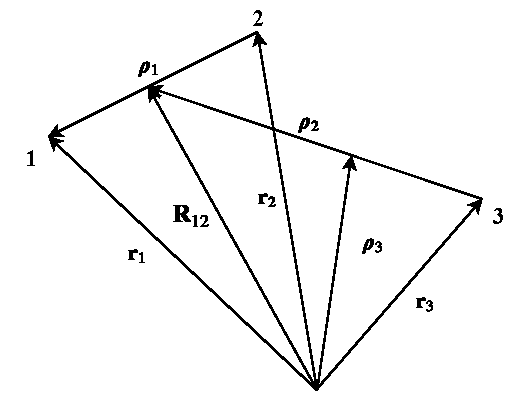
\includegraphics[width=0.5\linewidth]{pictures/jacobi_coordinates.pdf}
    \caption{Координаты Якоби  для системы из 3 частиц, пронумерованных 1, 2, 3. Через $\mf{R}_{12}$ бозначен вектор, направленный в центр масс пары частиц 1 и 2.}
    \label{fig:jacobi_coordinates}
\end{figure}

Можно показать, что кинетическая энергия в лагранжевой форме, выраженная через векторы Якоби записывается как \cite{greiner} 
\begin{gather}
    T_\text{tot} = \frac{1}{2} M \dot{\bs{\rho}}_N^2 + \frac{1}{2} \sum_{k = 1}^{N - 1} \mu_k \dot{\bs{\rho}}_k^2,
\end{gather}
%
где приведенные массы $\mu_j$ связаны с исходными массами $m_j$ следующими соотношениями
\begin{gather}
    \frac{1}{\mu_j} = \frac{1}{M_j} + \frac{1}{m_{j+1}}, \quad M_j = \sum_{k = 1}^j m_k, \quad j = 1 \dots N - 1. \label{polyatom-jacobi-masses}
\end{gather}

Данная последовательность введения векторов Якоби не является единственно возможной. Выбор векторов Якоби в каждом отдельном случае обусловлен структурой рассматриваемой системы. Описанная последовательность является общим случаем, в котором получена кинетическая энергия для системы из $N$ частиц. При другом выборе векторов Якоби общая форма кинетической энергии сохранится, однако изменятся приведенные массы $\mu_j$. \par
Отделяя центр масс, мы приходим к следующей форме кинетической энергии
\begin{gather}
    \Tl = \frac{1}{2} \sum_{k = 1}^{N - 1} \mu_k \dot{\bs{\rho}}_k^2.
\end{gather}

Для отделения вращательных степеней свободы введем подвижную систему координат. Лабораторная и подвижная системы координат связаны друг с другом матрицей ортогонального преобразования $\bbS$ \cite{goldstein}. Обозначим через $\mf{R}_j$ координаты векторов Якоби в подвижной системе координат. Введенные векторы $\mf{R}_j$ связаны с векторами в лабораторной системе линейным преобразованием
\begin{gather}
    \boldsymbol{\rho}_j = \bbS \mf{R}_j.
\end{gather}
Будем рассматривать параметризацию матрицы ортогонального преобразования $\bbS$ тройкой углов Эйлера $\Phi$, $\Theta$, $\Psi$ \cite{goldstein}
\begin{gather}
    \bbS = 
    \begin{bmatrix}
        \cos \Psi \cos \Phi - \cos \Theta \sin \Phi \sin \Psi & -\sin \Psi \cos \Phi - \cos \Theta \sin \Phi \cos \Psi & \sin \Theta \sin \Phi \\ 
        \cos \Psi \sin \Phi + \cos \Theta \cos \Phi \sin \Psi & -\sin \Psi \sin \Phi + \cos \Theta \cos \Phi \cos \Psi & - \sin \Theta \cos \Phi \\
        \sin \Theta \sin \Psi & \sin \Theta \cos \Psi & \cos \Theta
    \end{bmatrix}.
\end{gather}

Лагранжева кинетическая энергия в подвижной системе отсчета может быть записана как \cite{landau-volume1}
\begin{gather}
    \Tl = \frac{1}{2} \sum_{i = 1}^{N-1} \mu_i \dot{\mf{R}}_i^2 + \frac{1}{2} \sum_{i = 1}^{N - 1} \mu_i \lsq \boldsymbol{\Omega} \times \mf{R}_i \rsq^2 + \boldsymbol{\Omega}^{+} \sum_{i = 1}^{N - 1} \mu_i \lsq \mf{R}_i \times \dot{\mf{R}}_i \rsq,
\end{gather}
%
где $\boldsymbol{\Omega}$ -- вектор угловой скорости в проекции на подвижную систему координат. Вектор угловой скорости $\boldsymbol{\Omega}$ связан с углами Эйлера и эйлеровыми скоростями следующим соотношением
\begin{gather}
    \boldsymbol{\Omega} = \bbV \dot{\boldsymbol{\Upsilon}}_e = 
    \begin{bmatrix}
        \sin \Theta \sin \Psi & \cos \Psi & 0 \\
        \sin \Theta \cos \Psi & -\sin \Psi & 0 \\
        \cos \Theta & 0 & 1 
    \end{bmatrix}
    \begin{bmatrix}
        \dot{\Phi} \\ \dot{\Theta} \\ \dot{\Psi}
    \end{bmatrix}. \label{polyatom-matrixV}
\end{gather}

Введем набор внутренних координат $\mf{q} = \lb q_1, \dots q_s \rb$ и, используя связь координат Якоби с введенными координатами $\mf{R}_j = \mf{R}_j(\mf{q})$, перепишем выражение для кинетической энергии в форме \cite{petrov2015}
\begin{gather}
    \Tl = \frac{1}{2} \dot{\mf{q}}^+ \bba \dot{\mf{q}} + \bOmega^+ \bbA \mf{q} + \frac{1}{2} \bOmega^+ \bbI \, \bOmega, \label{body-fixed-lagrange-energy} 
\end{gather}
%
где через $\bba, \bbA, \bbI$ обозначены матрица относительной кинетической энергии, кориолисова матрица и матрица тензора инерции, соответственно. Элементы матриц относительной кинетической энергии и кориолисова взаимодействия заданы следующими выражениями
\begin{gather}
    \bba_{jk} = \sum_{i = 1}^{N - 1} \mu_i \frac{\partial \mf{R}_i}{\partial q_j} \frac{\partial \mf{R}_i}{\partial q_k}, \quad \bbA_{jk} = \sum_{i = 1}^{N - 1} \mu_i \lsq \mf{R}_i \times \frac{\partial \mf{R}_i}{\partial q_k} \rsq_j. \label{polyatom-kinetic-energy-matrices}
\end{gather}

Выражение для кинетической энергии \eqref{body-fixed-lagrange-energy} для перехода к Гамильтоновой форме удобно переписать в матричном виде
\begin{gather}
    \Tl = \frac{1}{2} \begin{bmatrix} \bOmega^+ & \dot{\mf{q}}^+ \end{bmatrix} \bbB \begin{bmatrix} \bOmega \\ \dot{\mf{q}} \end{bmatrix}, \label{polyatom-block-matrix-kin-energy}
\end{gather}
%
где через $\bbB$ обозначена блочная матрица со следующими элементами 
\begin{gather}
    \bbB = \begin{bmatrix} 
    \bbI & \bbA \\ \bbA^+ & \bba 
    \end{bmatrix}.
\end{gather}

Можно показать, что если ввести величину $\mf{J}$ как производную кинетической энергии в лагранжевой форме $\Tl$ по вектору угловой скорости $\bOmega$, то $\mf{J}$ суть вектор углового момента в подвижной системе координат (приложение \ref{appendix:angular-momentum-body-fixed}). Обобщенные импульсы $\mf{p}$, сопряженные координатам $\mf{q}$, по определению ранвы производным кинетической энергии в лагранжевой форме $\Tl$ по обобщенным скоростям $\dot{\mf{q}}$: 
\begin{gather}
    \mf{J} = \frac{\partial \Tl}{\partial \bOmega} = \bbI \bOmega + \bbA \dot{\mf{q}}, \label{polyatom-angmom1} \\
\mf{p} = \frac{\partial \Tl}{\partial \dot{\mf{q}}} = \bbA^+ \bOmega + \bba \dot{\mf{q}} \label{polyatom-gen-momenta}.
\end{gather}

Заметим, что выражения \eqref{polyatom-angmom1}, \eqref{polyatom-gen-momenta} могли быть получены дифференцированием выражения  \eqref{polyatom-block-matrix-kin-energy} по блочному вектору с компонентами $\bOmega$ и $\dot{\mf{q}}$. Выражения для углового момента и обобщенных импульсов объединим в один блочный вектор
\begin{gather}
    \begin{bmatrix} \mf{J} \\ \mf{p} \end{bmatrix} = \bbB \begin{bmatrix} \bOmega \\ \dot{\mf{q}} \end{bmatrix} = 
    \begin{bmatrix} \bbI & \bbA \\ \bbA^+ & \bba \end{bmatrix} \begin{bmatrix} \bOmega \\ \dot{\mf{q}} \end{bmatrix}.
\end{gather}

Для того, чтобы выразить лагранжевы переменные из полученного выражения, нам необходимо обратить блочную матрицу $\bbB$. Это обращение удобно выполнить при помощи формул Фробениуса \cite{petrov2015, gantmaher}. Через $\bbG$ обозначают обратную матрицу к $\bbB$, ее матричные компоненты выражаются как
\begin{gather}
    \begin{aligned}
        \bbG_{11} &= \lb \bbI - \bbA \bba^{-1} \bbA^+ \rb^{-1} \\
        \bbG_{12} &= -\bbI^{-1} \bbA \bbG_{22} = -\bbG_{11} \bbA \bba^{-1} \\
        \bbG_{21} &= -\bba^{-1} \bbA^+ \bbG_{11} = \bbG_{22} \bbA^+ \bbI^{-1} \\
        \bbG_{22} &= \lb \bba - \bbA^+ \bbI^{-1} \bbA \rb^{-1}
    \end{aligned} \label{polyatom-frobenius}
\end{gather}

Переход от кинетической энергии в форме Лагранжа к кинетической энергии в форме Гамильтона осуществляем при помощи стандартной процедуры \cite{goldstein}
\begin{gather}
    \Th = \begin{bmatrix} \bOmega^+ & \dot{\mf{q}}^+ \end{bmatrix} \begin{bmatrix} \mf{J} \\ \mf{p} \end{bmatrix} - \Tl = \frac{1}{2} \begin{bmatrix} \mf{J}^+ & \mf{p}^+ \end{bmatrix} \bbG \begin{bmatrix} \mf{J} \\ \mf{p} \end{bmatrix} = \frac{1}{2} \mf{J}^+ \bbG_{11} \mf{J} + \mf{J}^+ \bbG_{12} \mf{p} + \frac{1}{2} \mf{p}^+ \bbG_{22} \mf{p}, \label{general-rovibrational-kin-energy} 
\end{gather}
а полный колебательно-вращательный гамильтониан получается в результате добавления потенциальной энергии
\begin{gather}
    H = \frac{1}{2} \mf{J}^+ \bbG_{11} \mf{J} + \mf{J}^+ \bbG_{12} \mf{p} + \frac{1}{2} \mf{p}^+ \bbG_{22} \mf{p} + U(\mf{q}). \label{general-rovibrational-hamiltonian} 
\end{gather}

В данной работе мы будем рассматривать системы, состоящие из жесткой линейной молекулы атома и из двух жестких линейных молекул. \par
В случае системы линейная молекула$-$атом построим вектор Якоби вдоль линейной молекулы, тогда второй вектор Якоби соединяет центр масс линейной молекулы с атомом. Определим подвижную систему координат таким образом, чтобы построенные вектора Якоби $\mf{R}_1$, $\mf{R}_2$ задавали плоскость $OXZ$ подвижной системы. Дополнительно потребуем, чтобы вектор $\mf{R}_2$, соединяющий центр масс линейной молекулы с атомом, лежал вдоль оси $OZ$ (см. рис. \ref{fig:body-fixed-linear-atom}). Такое определение системы координат известно как $R$-вложение \cite{tennyson1986}. Обозначим длину линейной молекулы через $l$.
    
\begin{figure}[H]
    \centering
    %\begin{minipage}{0.49\linewidth}
    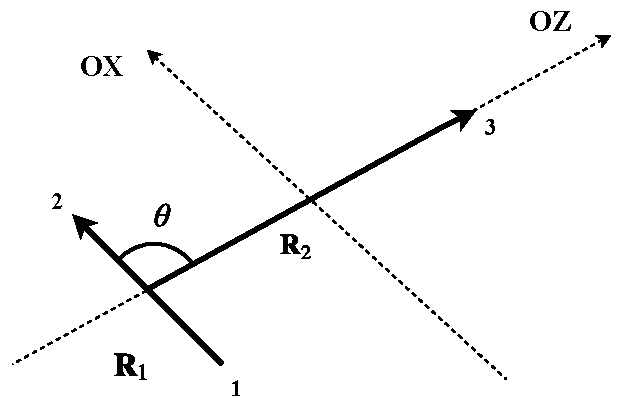
\includegraphics[width=0.5\linewidth]{pictures/triatom_coordinates.pdf}
    %\end{minipage}
    %\begin{minipage}{0.49\linewidth}
    %    Взять картинку из будущей статьи с N$_2$-N$_2$
    %\end{minipage}
    \caption{Молекулярная система координат для системы линейная молекула-атом}
    \label{fig:body-fixed-linear-atom}
\end{figure}

В качестве обобщенных координат выберем $R$ -- длину вектора Якоби $\mf{R}_2$ или, что эквивалентно, расстояние от атома до центра масс линейной молекулы, и угол $\theta$ между векторами Якоби $\mf{R}_1$ и $\mf{R}_2$. Угол $\theta$ отсчитывается от оси $OZ$ в сторону положительного направления оси $OX$, его область значений -- от $0$ до $\pi$. Выпишем координаты векторов в подвижной системе через обобщенные координаты $\mf{q} = \lb R, \theta \rb$: 
\begin{gather}
    \begin{aligned}
        X_1 &= l \sin \theta \\
        Y_1 &= 0 \\
        Z_1 &= l \cos \theta
    \end{aligned} \qquad
    \begin{aligned}
        X_2 &= 0 \\ 
        Y_2 &= 0 \\
        Z_2 &= R 
    \end{aligned}. \label{linear-molecule-atom-jacobi-coords}
\end{gather}

Вывод дальнейших выражений реализовывался в системе компьютерной алгебры Maple. Координаты векторов Якоби \eqref{linear-molecule-atom-jacobi-coords} использовались для расчета компонент матриц относительной кинетической энергии, кориолисова взаимодействия и тензора инерции по выражениям \eqref{polyatom-kinetic-energy-matrices}. В случае линейная молекула$-$атом блоки матрицы $\bbG$ могут быть получены в компактном виде. Уже для случая двух жестких линейных молекул выражения для блоков матрицы $\bbG$ оказываются слишком громоздкими, поэтому была разработана схема реализации траекторного расчета, избегающая аналитической работы с компонентами этих матриц, переносимая на системы с произвольным количеством вращательных степеней свободы. \par
В качестве примера системы линейная молекула$-$атом мы выбрали CO$_2-$Ar. Внутримолекулярные колебания молекулы CO$_2$ происходят существенно быстрее межмолекулярных движений комплекса с атомом аргона, поэтому предполагается, что взаимодействие между внутри- и межмолекулярными колебательными модами в данном случае компенсируется. \par
Приведенные массы частиц Якоби согласно \eqref{polyatom-jacobi-masses} равны
\begin{gather}
    \mu_1 = \frac{m_1}{2}, \quad \mu_2 = \frac{m_2 \lb 2 m_1 + m_3 \rb}{2 m_1 + m_2 + m_3},
\end{gather}
% 
где через $m_1$ обозначена масса атома кислорода, через $m_2$ -- масса атома аргона, через $m_3$ -- масса атома углерода. \par
При помощи системы компьютерной алгебры были получены следующие выражения для матриц кинетической энергии в форме Лагранжа
\begin{gather}
	\bba =
	\begin{bmatrix}
		\mu_2 & 0 \\
		0 & \mu_1 l^2
	\end{bmatrix}, \quad 
	\bbA = 
	\begin{bmatrix}
		0 & 0 \\
		0 & \mu_1 l^2 \\
		0 & 0 
	\end{bmatrix}, \quad
	\bbI = 
	\begin{bmatrix}
		\mu_1 l^2 \cos^2 \theta + \mu_2 R^2 & 0 & -\mu_1 l^2 \sin \theta \cos \theta \\
		0 & \mu_1 l^2 + \mu_2 R^2 & 0 \\
		- \mu_1 l^2 \sin \theta \cos \theta & 0 & \mu_1 l^2 \sin^2 \theta
	\end{bmatrix}. \notag
\end{gather}

Подставив полученные выражения для матриц в формулы Фробениуса \eqref{polyatom-frobenius}, приходим к следующим выражениям для матриц, определяющим кинетическую энергию в форме Гамильтона 
\begin{gather}
	\bbG_{11} =
	\begin{bmatrix}
		\dfrac{1}{\mu_2 R^2} & 0 & \dfrac{\ctg \theta}{\mu_2 R^2} \\
		0 & \dfrac{1}{\mu_2 R^2} & 0 \\
		\dfrac{\ctg \theta}{\mu_2 R^2} & 0 & \dfrac{\ctg^2 \theta}{\mu_2 R^2} + \dfrac{1}{\mu_1 l^2 \sin^2 \theta}
	\end{bmatrix}, \quad
	\bbG_{12} =
	\begin{bmatrix}
		0 & 0 \\
		0 & - \dfrac{1}{\mu_2 R^2} \\
		0 & 0
	\end{bmatrix}, \quad 
	\bbG_{22} = 
	\begin{bmatrix}
		\dfrac{1}{\mu_2} & 0 \\
		0 & \dfrac{1}{\mu_2 R^2} + \dfrac{1}{\mu_1 l^2}
	\end{bmatrix}. \notag
\end{gather}

Итак, кинетическая энергия в форме Гамильтона для системы CO$_2-$Ar в выбранной нами молекулярной системе отсчета получается следующей
\begin{gather}
\Th = \frac{1}{2 \mu_2} p_R^2 + \lb \frac{1}{2 \mu_2 R^2} + \frac{1}{2 \mu_1 l^2} \rb p_\theta^2 - \frac{1}{\mu_2 R^2} p_\theta \Jy + \frac{1}{2 \mu_2 R^2} \Jy^2 + \frac{1}{2 \mu_2 R^2} \Jx^2 + \frac{1}{2 \sin^2 \theta} \lb \frac{\cos^2 \theta}{\mu_2 R^2} + \frac{1}{\mu_1 l^2} \rb \Jz^2 + \notag \\
+ \frac{\ctg \theta}{\mu_2 R^2} \Jx \Jz. 
\end{gather}

В случае системы, состоящей из двух жестких линейных молекул, удобно построить векторы Якоби вдоль каждой из линейных молекул, тогда третий вектор соединяет их центры масс. Определим подвижную систему координат таким образом, чтобы вектор, соединяющий центры масс линейных молекул, лежал на оси $OZ$ подвижной системы. Потребуем, чтобы вектор, определяющий одну из линейных молекул, лежал в плоскости $OXZ$ подвижной системы (Рис. \ref{fig:two-linear-molecules-body-fixed}). Вторая молекула при этом может выходить из плоскости подвижной системы -- для того, чтобы описать ее ориентацию необходимо ввести два угла, тогда как для описания ориентации первой молекулы достаточно одного полярного угла. Введя таким образом систему координат мы заведомо сделали линейные молекулы неравноправными, так что соответствующие им координаты будут входить в кинетическую энергию неодинаковым образом. Обозначим длины линейных молекул через $l_1$ и $l_2$, соответственно. В качестве обобщенных координат выберем $R$ -- расстояние между центрами масс линейных молекул, $\theta_1$, $\theta_2$ -- полярные углы линейных молекул в плоскости $OXZ$, отсчитываемые от оси $OZ$ в сторону положительного направления оси $OX$, $\varphi$ -- угол между плоскостью $OXZ$ и плоскостью, заданной молекулой, выходящей из плоскости подвижной системы, и центром масс второй молекулы. Обобщенные координаты объединим в вектор $\mf{q} = \lb R, \varphi, \theta_1, \theta_2 \rb$. 

\begin{figure}[H]
    \centering
    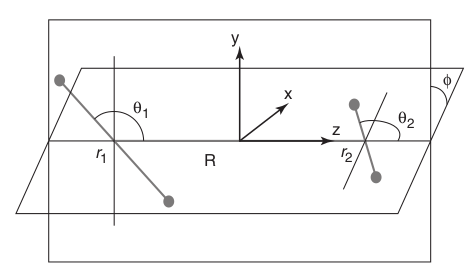
\includegraphics[width=0.5\linewidth]{pictures/n2n2_coordinate_frame.png}
    \caption{Молекулярная система координат для системы из двух линейных молекул; взять картинку из драфта статьи?}
    \label{fig:two-linear-molecules-body-fixed}
\end{figure}

Выпишем координаты векторы Якоби в подвижной системе через обобщенные координаты 
\begin{gather}
    \begin{aligned}
        X_1 &= l_1 \sin \theta_1 \\
        Y_1 &= 0 \\
        Z_1 &= l_1 \cos \theta_1 
    \end{aligned} \qquad
    \begin{aligned}
        X_2 &= l_2 \cos \varphi \sin \theta_2 \\
        Y_2 &= l_2 \sin \varphi \sin \theta_2 \\
        Z_2 &= l_2 \cos \theta_2
    \end{aligned} \qquad
    \begin{aligned}
        X_3 &= 0 \\
        Y_3 &= 0 \\
        Z_3 &= R
    \end{aligned} \label{polyatom-linear-linear-coordinates}
\end{gather}

В качестве примера системы, состоящей из двух линейных молекул, выбрана N$_2-$N$_2$. Приведенные масс частиц Якоби равны
\begin{gather}
    \mu_1 = \frac{m}{2}, \quad \mu_2 = \frac{m}{2}, \quad \mu_3 = 2m, \label{polyatom-n2n2-jacobi-masses}
\end{gather}
%
где через $m$ обозначена масса атома азота. Длины линейных молекул в дальнейшем обозначаются одинаково $l = l_1 = l_2$.

Выражения для матриц кинетической энергии в форме Лагранжа были получены из \eqref{polyatom-linear-linear-coordinates} при помощи системы компьютерной алгебры. Введенный набор координат является ортогональным, т.к. матрица относительной кинетической энергии оказывается диагональной. Приводим выражения для случая двух произвольных линейных молекул через массы частиц Якоби; выражения для конкретного случая N$_2-$N$_2$ получаются в результате подстановки масc \eqref{polyatom-n2n2-jacobi-masses}.  
\begin{gather}
\bba = 
\begin{bmatrix}
\mu_3 & 0 & 0 & 0 \\
0 & \mu_2 l_2^2 \sin^2 \theta_2 & 0 & 0 \\
0 & 0 & \mu_1 l_1^2 & 0 \\
0 & 0 & 0 & \mu_2 l_2^2 \\ 
\end{bmatrix}, \quad  
\bbA = 
\begin{bmatrix}
0 & -\mu_2 l_2^2 \cos \varphi \sin \theta_2 \cos \theta_2 & 0 & -\mu_2 l_2^2 \sin \varphi  \\
0 & -\mu_2 l_2^2 \sin \varphi \sin \theta_2 \cos \theta_2 & \mu_1 l_1^2 & \mu_2 l_2^2 \cos \varphi \\
0 &  \mu_2 l_2^2 \sin^2 \theta_2 & 0 & 0
\end{bmatrix} \notag 
\end{gather}

Компоненты матрицы тензора инерции в подвижной системе отсчета получаются следующие
\begin{gather}
    \begin{aligned}
        I_{XX} &= \mu_1 l_1^2 \cos^2 \theta_1 + \mu_2 l_2^2 (\sin^2 \varphi \sin^2 \theta_2 + \cos^2 \theta_2) + \mu_3 R^2, \\ 
        I_{XY} &= -\mu_2 l_2^2 \sin \varphi \cos \varphi \sin^2 \theta_2, \\ 
        I_{XZ} &= -\mu_1 l_1^2 \sin \theta_1 \cos \theta_1 - \mu_2 l_2^2 \cos \varphi \sin \theta_2 \cos \theta_2, \\
        I_{YY} &= \mu_1 l_1^2 + \mu_2 l_2^2 (\cos^2 \varphi \sin^2 \theta_2 + \cos^2 \theta_2) + \mu_3 R^2, \\
        I_{YZ} &= -\mu_2 l_2^2 \sin \varphi \sin \theta_2 \cos \theta_2, \\
        I_{ZZ} &= \mu_1 l_1^2 \sin^2 \theta_1 + \mu_2 l_2^2 \sin^2 \theta_2.  
    \end{aligned} 
\end{gather}

Как уже было сказано, выражения для блоков матрицы $\bbG$ в этом случае получаются слишком громоздкими для работы, поэтому не приводятся. Для реализации траекторного расчета нет необходимости получать аналитические выражения для этих матриц. 

\section{Уравнения относительного вращения молекулярной системы отсчета} \label{section:rotational-dynamics}

В отсутствии внешних сил угловой момент $\mf{j}$ в лабораторной системе координат является векторным интегралом движения. Компоненты вектора углового момента в подвижной системе отсчета связаны с компонентами в лабораторной системе матрицей $\bbS^{-1}$
\begin{gather}
    \mf{J} = \bbS^{-1} \mf{j}. \label{polyatom-j-connection}
\end{gather}

Производная вектора углового момента в подвижной системе удовлетворяет следующему соотношению \cite{goldstein}
\begin{gather}
    \dot{\mf{J}} + \lsq \bOmega \times \mf{J} \rsq = 0.
\end{gather}

Используя теорему Донкина можно показать \cite{petrov2015}, что 
\begin{gather}
    \bOmega = \frac{\partial \Th}{\partial \mf{J}}. 
\end{gather}

Таким образом, векторы угловой скорости и углового момента, не будучи сами динамическими переменными, связаны такими же соотношениями как канонически сопряженные переменные (так называемые \textit{псевдо-канонические переменные}):
\begin{gather}
    \mf{J} = \frac{\partial \Tl}{\partial \bOmega}, \qquad \bOmega = \frac{\partial \Th}{\partial \mf{J}}.
\end{gather}

Закон сохранения углового момента в подвижной системе координат преобразуется к уравнениям, называемым обобщенными уравнениями Эйлера \cite{petrov2015}
\begin{gather}
    \dot{\mf{J}} + \Big[ \frac{\partial \Th}{\partial \mf{J}} \times \mf{J} \Big] = 0. \label{generalized-euler-equations}
\end{gather}

Понятно, что модуль углового момента в подвижной системе отсчета является интегралом движения (в силу ортогональности преобразования в \eqref{polyatom-j-connection}). Следовательно, уравнения \eqref{generalized-euler-equations} можно преобразовать таким образом, чтобы учитывать сохранение модуля углового момента. Будем описывать ориентацию вектора углового момента в подвижной системе при помощи пары сферических углов $\alpha$ и $\beta$
\begin{gather}
    \begin{aligned}
        \Jx &= J \cos \alpha \sin \beta, \\
        \Jy &= J \sin \alpha \sin \beta, \\
        \Jz &= J \cos \beta.
    \end{aligned} \label{polyatom-angmom-spherical-coordinates}
\end{gather}

Получим соотношения между производными сферических координат и производными декартовых координат вектора углового момента. Для этого продифференцируем соотношения \eqref{polyatom-angmom-spherical-coordinates} по времени 
\begin{gather}
    \begin{aligned}
        \dot{\Jx} &= \dot{J} \cos \alpha \sin \beta - J \dot{\alpha} \sin \alpha \sin \beta + J \dot{\beta} \cos \alpha \cos \beta, \\
        \dot{\Jy} &= \dot{J} \sin \alpha \sin \beta + J \dot{\alpha} \cos \alpha \sin \beta + J \dot{\beta} \sin \alpha \cos \beta, \\
        \dot{\Jz} &= \dot{J} \cos \beta - J \dot{\beta} \sin \beta,
    \end{aligned}
\end{gather}

и разрешим их относительно сферических координат
\begin{gather}
    \begin{aligned}
        \dot{J} &= \dJx \cos \alpha \sin \beta + \dJy \sin \alpha \sin \beta + \dJz \cos \beta, \\
        \dot{\alpha} &= -\frac{\dJx \sin \alpha + \dJy \cos \alpha}{J \sin \beta}, \\
        \dot{\beta} &= \frac{\dJx \cos \alpha \cos \beta + \dJy \sin \alpha \cos \beta  - \dJz \sin \beta}{J}.
    \end{aligned} \label{polyatom-temp1}
\end{gather}

Подставив производные декартовых координат из \eqref{generalized-euler-equations} в соотношения \eqref{polyatom-temp1}, получим
\begin{gather}
    \begin{aligned}
        \dot{J} &= 0, \\
        \dot{\alpha} &= \lb \frac{\partial H}{\partial \Jx} \cos \alpha + \frac{\partial H}{\partial \Jy} \sin \alpha \rb \ctg \beta - \frac{\partial H}{\partial \Jz}, \\
        \dot{\beta} &= \frac{\partial H}{\partial \Jx} \sin \alpha - \frac{\partial H}{\partial \Jy} \cos \alpha.
    \end{aligned} \label{polyatom-temp2}
\end{gather}

Первое из уравнений \eqref{polyatom-temp2} говорит нам о сохранении модуля вектора углового момента в подвижной системе координат. Это уравнение мы отбросим, так как оно не дает нам ничего нового. Мы получили динамические уравнения для углов $\alpha$, $\beta$, но они содержат производные гамильтониана по декартовым компонентам углового момента. Чтобы получить замкнутые уравнения относительно сферических углов, выразим при помощи цепного правила производные гамильтониана по декартовым координаты через производные по сферическим координатам:    
\begin{gather}
    \begin{aligned}
        \frac{\partial H}{\partial \Jx} &= \sum_{\gamma = J, \alpha, \beta} \frac{\partial H}{\partial \gamma} \frac{\partial \gamma}{\partial \Jx}, \\
        \frac{\partial H}{\partial \Jy} &= \sum_{\gamma = J, \alpha, \beta} \frac{\partial H}{\partial \gamma} \frac{\partial \gamma}{\partial \Jy}, \\
        \frac{\partial H}{\partial \Jz} &= \sum_{\gamma = J, \alpha, \beta} \frac{\partial H}{\partial \gamma} \frac{\partial J_\gamma}{\partial \Jz}.
    \end{aligned} \label{polyatom-temp3}
\end{gather}

Соотношения \eqref{polyatom-temp3} удобнее представить в матричном виде. Вычислив производные сферических координат по декартовым, приходим к следующим соотношениям
\begin{gather}
    \begin{bdmatrix}
        \frac{\partial H}{\partial \Jx} \\
        \frac{\partial H}{\partial \Jy} \\
        \frac{\partial H}{\partial \Jz}
    \end{bdmatrix} = \bbF 
    \begin{bdmatrix}
        \frac{\partial H}{\partial J} \\
        \frac{\partial H}{\partial \alpha} \\
        \frac{\partial H}{\partial \beta}
    \end{bdmatrix}, \qquad 
    \bbF = 
    \begin{bdmatrix}
        \cos \alpha \sin \beta & - \frac{1}{J} \frac{\sin \alpha}{\sin \beta} & \frac{1}{J} \cos \alpha\ \cos \beta \\ 
        \sin \alpha \sin \beta & \frac{1}{J} \frac{\cos \alpha}{\sin \beta} & \frac{1}{J} \sin \alpha \cos \beta \\
        \cos \beta & 0 & -\frac{1}{J} \sin \beta
    \end{bdmatrix}. \label{polyatom-temp4}
\end{gather}

Подставив уравнения \eqref{polyatom-temp4} в динамические уравнения \eqref{polyatom-temp2}, приходим к динамическим уравнениям, замкнутым относительно сферических переменных:
\begin{gather}
    \begin{aligned}
        \dot{\alpha} &= \frac{1}{J \sin \beta} \frac{\partial H}{\partial \beta}, \\
        \dot{\beta} &= - \frac{1}{J \sin \beta} \frac{\partial H}{\partial \alpha}.
    \end{aligned} \label{generalized-euler-equations-angles}
\end{gather}

Кроме того, уравнения вращательной динамики могут быть написаны относительно углов Эйлера $\bUpsilon = \lb \Phi, \Theta, \Psi \rb$ и сопряженных к ним импульсов $\pe = \lb p_\Phi, p_\Theta, p_\Psi \rb$. Так как они являются набором канонически сопряженных переменных, то в этом случае уравнения вращательной динамики будут представлять собой два векторных уравнения Гамильтона
\begin{gather}
    \begin{aligned}
        \dot{\boldsymbol{\Upsilon}}_e &= \frac{\partial \Th}{\partial \pe}, \\
        \dot{\mathbf{p}}_e &= -\frac{\partial \Th}{\partial \bUpsilon}.
    \end{aligned} \label{euler-hamilton-equations}
\end{gather}

Итак, для описания вращательной динамики у нас имеется три разных системы динамических уравнений:
\begin{enumerate}
    \item Обобщенные уравнения Эйлера, записанные в компонентах углового момента \eqref{generalized-euler-equations}
    \item Преобразованные обобщенные уравнения Эйлера, в которых учтено сохранение модуля вектора углового момента в молекулярной системе координат \eqref{generalized-euler-equations-angles}
    \item Уравнения, записанные в эйлеровых углах и сопряженных к ним импульсах \eqref{euler-hamilton-equations}
\end{enumerate}

Система уравнений \eqref{generalized-euler-equations-angles} содержит наименьшее возможное количество уравнений для описания вращения. Однако введение сферической системы вводит в систему уравнений два полюса -- $\beta = 0$ и $\beta = \pi$. При этих значениях полярного угла, правые части уравнений принимают бесконечные значения, хотя они отвечают физически реализуемым положениям полного углового момента вдоль положительного или отрицательного направлений оси $OZ$ подвижной системы. Эту особенность сферической системы несложно преодолеть при построении вычислительной процедуре. Уравнения \eqref{generalized-euler-equations-angles} выписаны таким образом, что выделенной осью является ось $OZ$. Не представляет труда выписать аналогичную систему уравнений таким образом, чтобы выделенной осью была ось $OX$ или $OY$. Пусть в таком случае вращательными переменными будут $\alpha^\prime$ и $\beta^\prime$. Положение углового момента вдоль оси $OZ$ для таким образом построенной сферической системы не является особым. При численном интегрировании уравнений \eqref{generalized-euler-equations-angles} в случае приближения решения к одному из полюсов следует пересчитать угловые переменные $\alpha$, $\beta$ в переменные $\alpha^\prime$, $\beta^\prime$ и продолжить решение уже системы уравнений, построенной с другой выделенной осью. При прохождении полюса можно пересчитать вращательные переменные обратно и продолжить интегрирование в переменных $\alpha$, $\beta$. \par
Среди двух векторных уравнений \eqref{euler-hamilton-equations} содержится одно тривиальное уравнение. Рассмотрим выражение для эйлеровых импульсов $\pe$
\begin{gather}
    \pe = \frac{\partial \Tl}{\partial \dot{\boldsymbol{\Upsilon}}_e} = \frac{\partial \bOmega}{\partial \dot{\boldsymbol{\Upsilon}}_e} \frac{\partial \Tl}{\partial \bOmega} = \bbV^+ \mf{J}.
\end{gather}

Следовательно, вектор углового момента связан с вектором эйлеровых импульсов $\pe$ соотношением
\begin{gather}
    \mf{J} = \bbW \pe, \label{polyatom-angular-momentum-euler-momenta}
\end{gather}
%
где через $\bbW$ обозначена матрица $\lb \bbV^{+} \rb^{-1}$. Выражения для компонент матрицы $\bbV$ приведены в формуле \eqref{polyatom-matrixV}. Заметим, что эйлеров угол $\Phi$ не содержится в выражениях для компонент матрицы $\bbV$, следовательно, матрица $\bbW$ также не зависит от угла $\Phi$. Таким образом, угол $\Phi$ не содержится в общем колебательно-вращательном гамильтониане \eqref{general-rovibrational-hamiltonian}, откуда следует, что сопряженный импульс $p_\Phi$ является интегралом движения. \par

\section{Полные системы динамических уравнений и обращение классических траекторий}

В предыдущем параграфе мы рассматривали вопрос общего вида уравнений, описывающих вращение молекулярной системы отсчета. Для получения полной системы динамических уравнений эти уравнения должны быть дополнены гамильтоновыми уравнениями по переменным $\mf{q}$ и $\mf{p}$
\begin{gather}
    \begin{aligned}
        \dot{\mf{q}} &= \frac{\partial H}{\partial \mf{p}}, \\
        \dot{\mf{p}} &= -\frac{\partial H}{\partial \mf{q}}.
    \end{aligned} \label{hamilton-equations}
\end{gather}

Рассмотрим структуру гамильтоновых уравнений \eqref{hamilton-equations} с гамильтонианом в форме \eqref{general-rovibrational-hamiltonian}. Отметим, что блоки матрицы $\bbG$ являются функциями обобщенных координат $\mf{q}$:
\begin{gather}
    \begin{aligned}
        \frac{\partial H}{\partial \mf{p}} &= \bbG_{22} \mf{p} + \bbG_{12}^{+} \mf{J}, \\
        \frac{\partial H}{\partial \mf{q}} &= \frac{1}{2} \mf{p}^+ \frac{\partial \bbG_{22}}{\partial \mf{q}} \mf{p} + \mf{J}^+ \frac{\partial \bbG_{12}}{\partial \mf{q}} \mf{p} + \frac{1}{2} \mf{J}^+ \frac{\partial \bbG_{11}}{\partial \mf{q}} \mf{J} + \frac{\partial U}{\partial \mf{q}}.
    \end{aligned} \label{hamilton-equations1}
\end{gather}

Для того, чтобы построить вычислительную процедуру для численного интегрирования уравнений \eqref{hamilton-equations1} мы должны получить выражения, по которым можно осуществлять расчет правых частей в произвольной точке фазового пространства $\lb \mf{q}_0, \mf{p}_0, \mf{J}_0 \rb$. Заметим, что формулы Фробениуса \eqref{polyatom-frobenius}, представляющие сложность при получении аналитических выражений для блоков матрицы $\bbG$, оказываются очень удобными, если матрицы $\bba$, $\bbA$, $\bbI$ оказываются числовыми матрицами. Для систем линейная молекула$-$атом и пара линейных молекул выражения для матриц лагранжевой кинетической энергии оказываются в достаточной степени простыми, и их вывод может быть в существенной степени автоматизирован при помощи системы компьютерной алгебры. Числовые значения компонент этих матриц определяются лишь значениями обобщенных координат $\mf{q}_0$. Вычислив по полученным выражениям численные значения компонент матрицы $\bba(\mf{q}_0)$, $\bbA(\mf{q}_0)$, $\bbI(\mf{q}_0)$, получаем значения матриц $\bbG_{11}(\mf{q}_0)$, $\bbG_{12}(\mf{q}_0)$, $\bbG_{22}(\mf{q}_0)$ по формулам Фробениуса. Таким образом, вычисление вектора производных $\partial H / \partial \mf{p}$ в произвольной точке не представляет сложности. \par
Рассмотрим вопрос дифференцирования блоков матрицы $\bbG$ по обобщенным координатам. Пусть $\bbM(\mf{q})$ -- дифференцируемая, обратимая матричная функция векторного аргумента $\mf{q}$. Производная обратной матрицы $\bbM^{-1}(\mf{q})$ по векторной переменной $\mf{q}$ связана с производной $\bbM^\prime(\mf{q})$ следующим соотношением \cite{matrixcookbook}
\begin{gather}
    \frac{\partial}{\partial \mf{q}} \bbM^{-1}(\mf{q}) = - \bbM^{-1}(\mf{q}) \bbM^\prime(\mf{q}) \bbM^{-1}(\mf{q}).
\end{gather}

Применим это соотношения для дифференцирования матрицы $\bbG_{11}(\mf{q})$ по вектору обобщенных координат $\mf{q}$
\begin{gather}
    \frac{\partial}{\partial \mf{q}} \bbG_{11} = \frac{\partial}{\partial \mf{q}} \lsq \lb \bbI - \bbA \bba^{-1} \bbA^+ \rb^{-1} \rsq = -\bbG_{11} \lsq \frac{\partial}{\partial \mf{q}} \lb \bbI - \bbA \bba^{-1} \bbA^+ \rb \rsq \bbG_{11} = \notag \\
    = -\bbG_{11} \lsq \frac{\partial \bbI}{\partial \mf{q}} - \frac{\partial \bbA}{\partial \mf{q}} \bba^{-1} \bbA^+ + \bbA \bba^{-1} \frac{\partial \bba}{\partial \mf{q}} \bba^{-1} \bbA^+ - \bbA \bba^{-1} \frac{\partial \bbA^+}{\partial \mf{q}} \rsq \bbG_{11}. \label{polyatom-g11-derivative}
\end{gather}
Аналогично, несложно получить выражения производных матриц $\bbG_{22}(\mf{q})$ и $\bbG_{12}(\mf{q})$:
\begin{gather}
    \frac{\partial}{\partial \mf{q}} \bbG_{22} = -\bbG_{22} \left[ \frac{\partial \bba}{\partial \mf{q}} - \frac{\partial \bbA^\top}{\partial \mf{q}} \bbI^{-1} \bbA + \bbA^\top \bbI^{-1} \frac{\partial \, \bbI}{\partial \mf{q}} \bbI^{-1} \bbA - \bbA^\top \bbI^{-1} \frac{\partial \bbA}{\partial \mf{q}} \right] \bbG_{22}, \label{polyatom-g22-derivative} \\
	\frac{\partial}{\partial \mf{q}} \bbG_{12} = - \left [ \frac{\partial}{\partial \mf{q}} \bbG_{11} \right] \bbA \bba^{-1} - \bbG_{11} \frac{\partial \bbA}{\partial \mf{q}} \bba^{-1} + \bbG_{11} \bbA \bba^{-1} \frac{\partial \bba}{\partial \mf{q}} \bba^{-1} = \notag \\
    = \bbG_{22} \left[ \frac{\partial \bba}{\partial \mf{q}} - \frac{\partial \bbA^\top}{\partial \mf{q}} \bbI^{-1} \bbA + \bbA^\top \bbI^{-1} \frac{\partial \, \bbI}{\partial \mf{q}} \bbI^{-1} \bbA - \bbA^\top \bbI^{-1} \frac{\partial \bbA}{\partial \mf{q}} \right] \bbG_{22} \bbA \bba^{-1} - \bbG_{11} \frac{\partial \bbA}{\partial \mf{q}} \bba^{-1} + \bbG_{11} \bbA \bba^{-1} \frac{\partial \bba}{\partial \mf{q}} \bba^{-1}. \label{polyatom-g12-derivative} 
\end{gather}

Таким образом, получив аналитические выражения для матриц $\bba$, $\bbA$, $\bbI$ и их производных по координатам $\mf{q}$, соотношения \eqref{polyatom-g11-derivative}, \eqref{polyatom-g22-derivative}, \eqref{polyatom-g12-derivative} позволяют вычислять производные блоков матрицы $\bbG$. Эти вычисления, разумеется, следует проводить уже с численными матрицами, т.к. аналитические выражения получаются слишком громоздкими для манипулирования. \par
Итак, мы описали схему вычисления правых частей уравнений \eqref{hamilton-equations1} на основе матриц, определяющих кинетическую энергию в Лагранжевой форме и их производных. Дополним уравнения \eqref{hamilton-equations1} уравнениями вращательной динамики, рассмотренными в параграфе \ref{section:rotational-dynamics}, и рассмотрим вид правых частей этих уравнений с колебательно-вращательным гамильтонианом вида \eqref{general-rovibrational-hamiltonian}. \par
Инверсия времени в классической траектории является одним из способов проверки ее качества. Для этого рассчитываем классическую траекторию в положительную сторону временной оси до достижения заданного расстояния между молекулами. Затем, используя соотношения между динамическими переменными при пропагировании траектории в положительную и отрицательную сторону по времени, осуществляем эффективную инверсию временной оси. Продемонстрируем обращение траекторий рассеяния на примере системы N$_2-$N$_2$. 

\subsection{Полная система динамических уравнений с углами Эйлера и сопряженными импульсами}
    Полная система уравнений с углами Эйлера и сопряженными импульсах состоит из $2s + 5$ уравнений (с учетом интеграла движения $p_\Phi$), где $s$ -- количество обобщенных координат $\mf{q}$:
\begin{gather}
    \begin{aligned}
        &\dot{\mf{q}} = \frac{\partial H}{\partial \mf{p}}, \\
        &\dot{\mf{p}} = -\frac{\partial H}{\partial \mf{q}}, \\
        &\dot{\boldsymbol{\Upsilon}}_e = \frac{\partial H}{\partial \pe}, \\
        &\dot{\mf{p}}_e = - \frac{\partial H}{\partial \bUpsilon},
    \end{aligned} \label{full-system-euler}
\end{gather}
%
в которых гамильтониан используется в следующей форме
\begin{gather}
    H = \frac{1}{2} \mf{p}^+ \bbG_{22} \mf{p} + \mf{p}^+_e \bbW^+ \bbG_{12} \mf{p} + \frac{1}{2} \mf{p}^+_e \bbW^+ \bbG_{11} \bbW \pe + U(\mf{q}). \label{general-rovibrational-hamiltonian-euler}
\end{gather}

Отдельно рассмотрим только последнее уравнение системы \eqref{full-system-euler}, т.к. остальные легко получаются c применением векторного анализа. 
\begin{gather}
    \frac{\partial H}{\partial \bUpsilon} = \mf{p}_e^+ \frac{\partial \bbW^+}{\partial \bUpsilon} \bbG_{12} \mf{p} + \frac{1}{2} \mf{p}_e^+ \frac{\partial \bbW^+}{\partial \bUpsilon} \bbG_{11} \bbW \pe + \frac{1}{2} \mf{p}_e^+ \bbW^+ \bbG_{11} \frac{\partial \bbW}{\partial \bUpsilon} \pe \label{polyatom-temp5} 
\end{gather}

Заметим, что если рассмотреть выражение \eqref{polyatom-temp5} покомпонентно, то второе и третье слагамое переходят друг в друга при транспонировании, следовательно, они равны. Осуществив алгебраические преобразования, приходим к следующему выражению: 
\begin{gather}
    \frac{\partial H}{\partial \bUpsilon} = \mf{p}_e^+ \frac{\partial \bbW^+}{\partial \bUpsilon} \lb \bbG_{12} \mf{p} + \bbG_{11} \bbW \pe \rb = \mf{p}_e^+ \frac{\partial \bbW^+}{\partial \bUpsilon} \bbV \frac{\partial H}{\partial \pe}.
\end{gather}

Конечная форма полного набора динамических уравнений в углах Эйлера выглядит следующим образом
\begin{gather}
    \begin{aligned}
        &\dot{\mf{q}} = \bbG_{22} \mf{p} + \bbG_{12}^+ \bbW \pe, \\
        &\dot{\mf{p}} = -\frac{1}{2} \mf{p}^+ \frac{\partial \bbG_{22}}{\partial \mf{q}} \mf{p} - \mf{p}_e^+ \bbW^+ \frac{\partial \bbG_{12}}{\partial \mf{q}} \mf{p} - \frac{1}{2} \mf{p}_e^+ \bbW^+ \frac{\partial \bbG_{11}}{\partial \mf{q}} \bbW \pe - \frac{\partial U}{\partial \mf{q}}, \\
        &\dot{\boldsymbol{\Upsilon}}_e = \bbW^+ \bbG_{11} \bbW \pe + \bbW^+ \bbG_{12} \mf{p}, \\
        &\dot{\mf{p}}_e = - \mf{p}_e^+ \frac{\partial \bbW^+}{\partial \bUpsilon} \lb \bbG_{12} \mf{p} + \bbG_{11} \bbW \pe \rb,
    \end{aligned} \label{polyatom-euler-system}
\end{gather}
%
где тензор третьего ранга $\partial \bbW^+ / \partial \bUpsilon$ может быть рассмотрен как вектор матриц c компонентами
\begin{gather}
	\frac{\partial \bbW}{\partial \varphi} = 0, \quad 
	\frac{\partial \bbW}{\partial \theta} = 
	\begin{bdmatrix}
		-\frac{\cos \theta \sin \psi}{\sin^2 \theta} & 0 & \frac{\sin \psi}{\sin^2 \theta} \\
		- \frac{\cos \theta \cos \psi}{\sin^2 \theta} & 0 & \frac{\cos \psi}{\sin^2 \theta} \\
		0 & 0 & 0
	\end{bdmatrix}, \quad 
	\frac{\partial \bbW}{\partial \psi} = 
	\begin{bdmatrix}
		\frac{\cos \psi}{\sin \theta} & - \sin \psi & -\frac{\cos \theta \cos \psi}{\sin \theta} \\
		- \frac{\sin \psi}{\sin \theta} & - \cos \psi & \frac{\cos \theta \sin \psi}{\sin \theta} \\
		0 & 0 & 0
	\end{bdmatrix}.
\end{gather}

Преобразование динамических переменных при инверсии времени $t \rightarrow -t$ задано следущими соотношениями
\begin{gather}
    \mf{q}(t) = \mf{q}(-t), \quad \mf{p}(t) = -\mf{p}(-t), \quad \bUpsilon(t) = \bUpsilon(-t), \quad \pe(t) = -\pe (-t). 
\end{gather}

На рис. (\ref{fig:euler-trajectory}) представлена траектория, полученная прямым пропагированием во времени, и траектория, полученная обратным пропагированием во времени из конечной точки прямой траектории. Мы видим, что они совпадают на протяжении 10-15 колебаний по радиальной координате. Это демонстрирует порядок точности траекторий, получающихся при решении системы \eqref{polyatom-euler-system}. На траекториях, в которых наблюдается больше 10-15 колебаний по радиальной координате, накапливаются существенные численные ошибки, которые приводят к нарушению инвариантности относительно инверсии времени.

\begin{figure}[H]
    \centering
    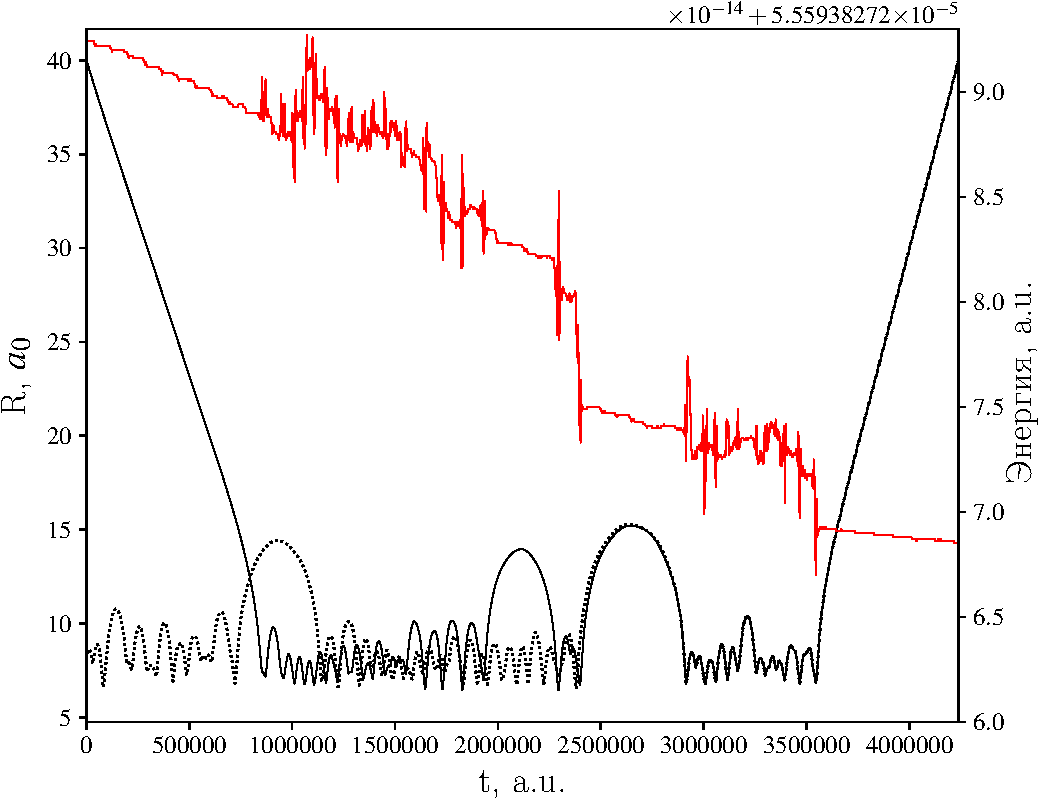
\includegraphics[width=0.75\linewidth]{./pictures/trajectories/euler_trajectory-crop.pdf}
\caption{Зависимости $R(t)$ для прямой (сплошная линия) и обратной (точечная линия) образования метастабильного комплекса N$_2-$N$_2$, полученные при решении полной системы динамических уравнений с углами и импульсами Эйлера \eqref{polyatom-euler-system}. Сверху отражено изменение энергии вдоль прямой траектории со шкалой справа.}
    \label{fig:euler-trajectory}
\end{figure}

\subsection{Полная система динамических уравнений с компонентами углового момента}
    Полная система динамических уравнений с компонентами углового момента содержит два уравнения Гамильтона относительно $\mf{q}$ и $\mf{p}$, дополненных обобщенным уравнением Эйлера, что в итоге приводит к системе из $2s + 3$ уравнений
\begin{gather}
    \begin{aligned}
        &\dot{\mf{q}} = \frac{\partial H}{\partial \mf{p}}, \\
        &\dot{\mf{p}} = -\frac{\partial H}{\partial \mf{q}}, \\
        &\dot{\mf{J}} + \Big[ \frac{\partial H}{\partial \mf{J}} \times \mf{J} \Big] = 0.
    \end{aligned}
\end{gather}

При подстановке колебательно-вращательного гамильтониана в форме \eqref{general-rovibrational-hamiltonian} приходим к следующему виду динамических уравнений
\begin{gather}
    \begin{aligned}
        &\dot{\mf{q}} = \bbG_{22} \mf{p} + \bbG_{12}^+ \mf{J}, \\
        &\dot{\mf{p}} = -\frac{1}{2} \mf{p}^+ \frac{\partial \bbG_{22}}{\partial \mf{q}} \mf{p} - \mf{J}^+ \frac{\partial \bbG_{12}}{\partial \mf{q}} \mf{p} - \frac{1}{2} \mf{J}^+ \frac{\partial \bbG_{11}}{\partial \mf{q}} \mf{J} - \frac{\partial U}{\partial \mf{q}}, \\
        &\dJx = \Jy \lb \bbG_{12} \mf{p} + \bbG_{11} \mf{J} \rb_z - \Jz \lb \bbG_{12} \mf{p} + \bbG_{11} \mf{J} \rb_y \\
        &\dJy = \Jz \lb \bbG_{12} \mf{p} + \bbG_{11} \mf{J} \rb_x - \Jx \lb \bbG_{12} \mf{p} + \bbG_{11} \mf{J} \rb_z \\
        &\dJz = \Jx \lb \bbG_{12} \mf{p} + \bbG_{11} \mf{J} \rb_y - \Jy \lb \bbG_{12} \mf{p} + \bbG_{11} \mf{J} \rb_x \\
    \end{aligned} \label{polyatom-jcomponents-system}
\end{gather}

Угловой момент $\mf{J}$ линейно связан с эйлеровыми импульсами согласно соотношению \eqref{polyatom-angular-momentum-euler-momenta}. При инверсии времени эйлеровы углы $\bUpsilon$ сохраняются, а эйлеровы импульсы меняют знак, следовательно вектор углового момента также претерпевает инверсию  
\begin{gather}
    \mf{q}(t) = \mf{q}(-t), \quad \mf{p}(t) = -\mf{p}(-t), \quad \mf{J}(t) = -\mf{J}(-t).
\end{gather}

Начальные условия для траектории, представленной на рис. (\ref{fig:jcomponents-trajectory}), были пересчитаны из начальных условий траектории на рис. (\ref{fig:euler-trajectory}). 

\begin{figure}[H]
    \centering
    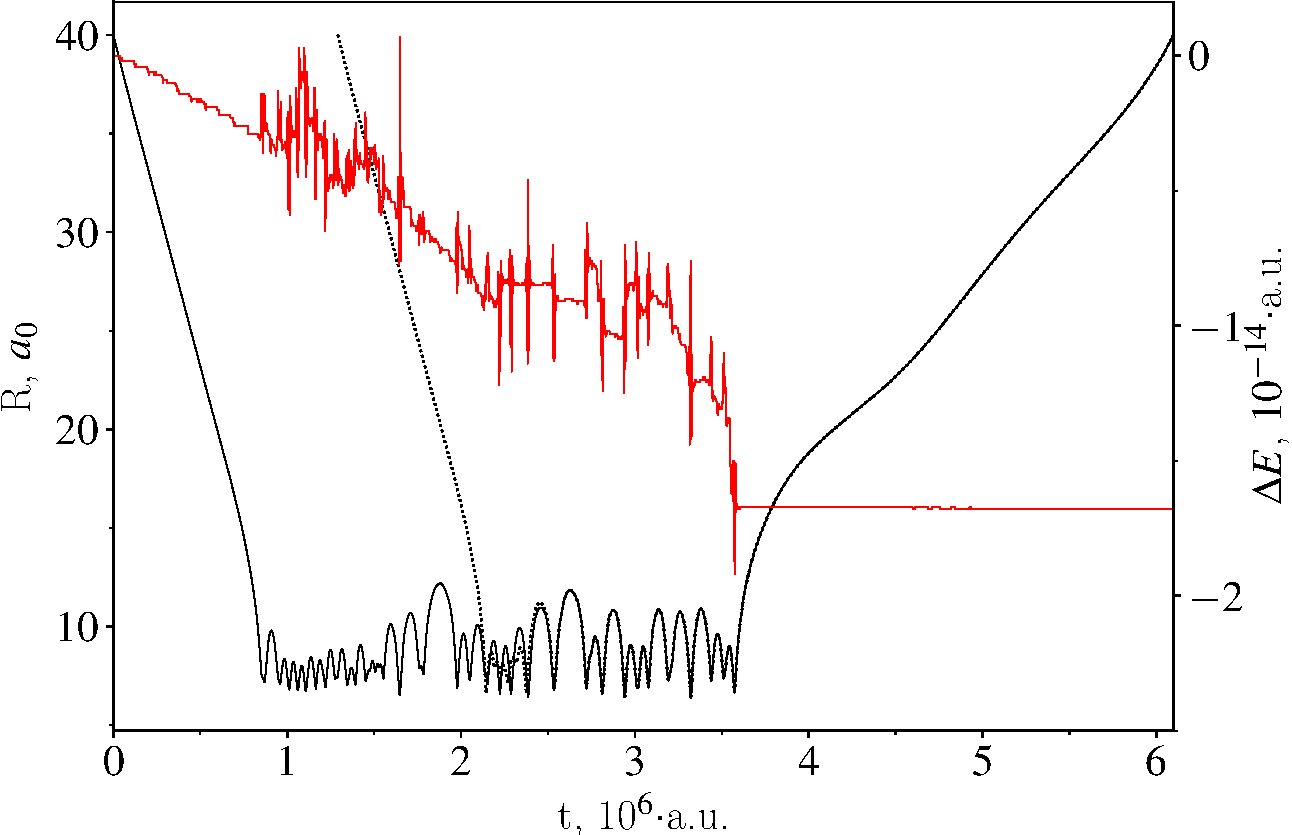
\includegraphics[width=0.75\linewidth]{./pictures/trajectories/jcomponents-trajectory-crop.pdf}
    \caption{Зависимости $R(t)$ для прямой (сплошная линия) и обратной (точечная линия) образования метастабильного комплекса N$_2-$N$_2$, полученные при решении полной системы динамических уравнений с декартовыми компонентами углового момента \eqref{polyatom-jcomponents-system}. Сверху отражено изменение энергии вдоль прямой траектории со шкалой справа.}
    \label{fig:jcomponents-trajectory}
\end{figure}


\subsection{Полная система динамических уравнений со сферическими углами углового момента}
В этом случае система уравнений состоит из двух векторных уравнений Гамильтона относительно $\mf{q}$, $\mf{p}$, дополненная двумя уравнениями относительно сферических углов углового момента $\alpha$ и $\beta$, что в сумме приводит к системе из $2s + 2$ уравнений
\begin{gather}
    \begin{aligned}
        &\dot{\mf{q}} = \frac{\partial H}{\partial \mf{p}}, \\
        &\dot{\mf{p}} = -\frac{\partial H}{\partial \mf{q}}, \\
        &\dot{\alpha} = \frac{1}{J \sin \beta} \frac{\partial H}{\partial \beta}, \\
        &\dot{\beta} = -\frac{1}{J \sin \beta} \frac{\partial H}{\partial \alpha}.
    \end{aligned}
\end{gather}

Подставив колебательно-вращательный гамильтониан в форме \eqref{general-rovibrational-hamiltonian}, приходим к следующей системе уравнений
\begin{gather}
    \begin{aligned}
        &\dot{\mf{q}} = \bbG_{22} \mf{p} + \bbG_{12}^+ \mf{J}, \\
        &\dot{\mf{p}} = -\frac{1}{2} \mf{p}^+ \frac{\partial \bbG_{22}}{\partial \mf{q}} \mf{p} - \mf{J}^+ \frac{\partial \bbG_{12}}{\partial \mf{q}} \mf{p} - \frac{1}{2} \mf{J}^+ \frac{\partial \bbG_{11}}{\partial \mf{q}} \mf{J} - \frac{\partial U}{\partial \mf{q}}, \\
        &\dot{\alpha} = \frac{1}{J \sin \beta} \lsq \bbF \lb \bbG_{11} \mf{J} + \bbG_{12} \mf{p} \rb \rsq_y, \\
        &\dot{\beta} = -\frac{1}{J \sin \beta} \lsq \bbF \lb \bbG_{11} \mf{J} + \bbG_{12} \mf{p} \rb \rsq_z, 
    \end{aligned} \label{polyatom-jspherical-system}
\end{gather}
%
где компоненты вектора углового момента равны $\mf{J} = \lb J \cos \alpha \sin \beta, J \sin \alpha \sin \beta, J \cos \beta \rb$. \par
Исходя из того, что при обращении времени происходит инверсия вектора углового момента, несложно получить следующие преобразования сферических углов вектора углового момента
\begin{gather}
    \mf{q}(t) = \mf{q}(-t), \quad \mf{p}(t) = -\mf{p}(-t), \quad \alpha(t) = \alpha(-t) - \pi, \quad \beta(t) = \pi - \beta(-t).
\end{gather}

Начальные условия для траектории, представленной на рис. (\ref{fig:jspherical-trajectory}), были пересчитаны из начальных условий траектории на рис. (\ref{fig:euler-trajectory}). 

\begin{figure}[H]
    \centering
    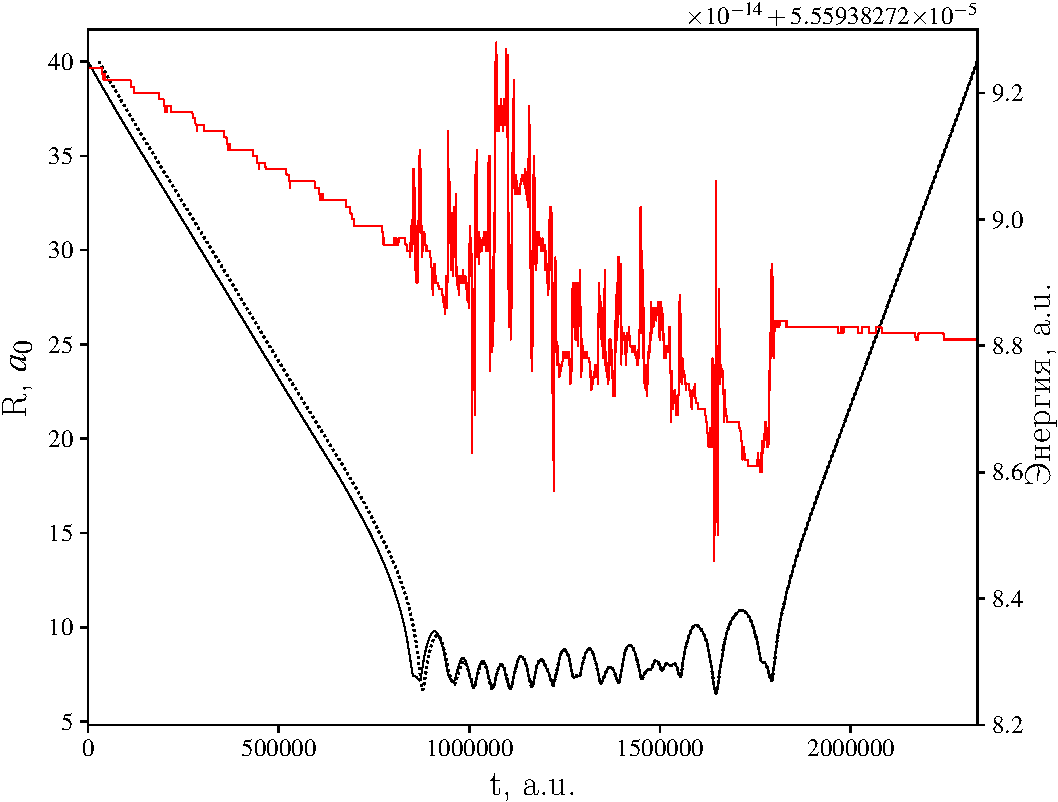
\includegraphics[width=0.75\linewidth]{./pictures/trajectories/spherical_trajectory-crop.pdf}
    \caption{Зависимости $R(t)$ для прямой (сплошная линия) и обратной (точечная линия) образования метастабильного комплекса N$_2-$N$_2$, полученные при решении полной системы динамических уравнений со сферическими углами углового момента \eqref{polyatom-jspherical-system}. Сверху отражено изменение энергии вдоль прямой траектории со шкалой справа.}
    \label{fig:jspherical-trajectory}
\end{figure}

На рис. (\ref{fig:trajectory-comparison}) представлено сравнение траекторий, пропагируемых в прямую сторону по времени, полученных при интегрировании трех разных систем уравнений. Мы видим, что интервал совпадения траекторий между собой сопоставим с интервалом совпадения прямой и обратной траекторий, полученных для каждой системы по отдельности. Таким образом, накопление численных ошибок происходит с сопоставимой скоростью для всех трех систем уравнений, поэтому никакую из систем нельзя выделить как более предпочтительную. \par

\begin{figure}[H]
    \centering
    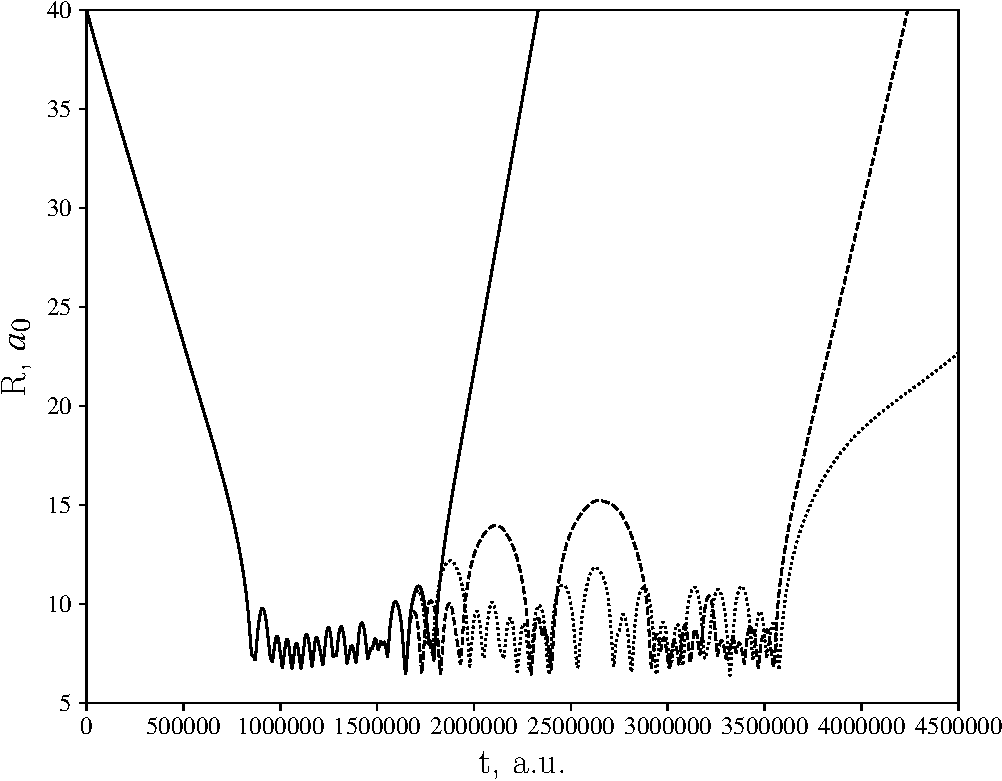
\includegraphics[width=0.75\linewidth]{./pictures/trajectories/trajectory-comparison-crop.pdf}
    \caption{Зависимости $R(t)$ образования метастабильного комплекса, полученные при решении системы динамических уравнений с углами Эйлера (сплошная линия), системы с компонентами углового момента (точечная линия), системы со сферическими углами углового момента (пунктирная линия).}
    \label{fig:trajectory-comparison}
\end{figure}

Кроме того, при интегрировании траекторий на рис. \ref{fig:trajectory-comparison} были сделаны замеры количества промежуточных вычислений правых частей уравнений. Количество вызовов правых частей для пропагирования траекторий до фиксированного времени (1.500.000 атомных единиц времени) отличается не более чем на 1\%. Вычисление кинетической части для системы со сферическими углами углового момента \eqref{polyatom-jspherical-system} оказывается в среднем быстрее на 5-7\%, чем вычисление кинетической части для системы с декартовыми компонентами углового момента \eqref{polyatom-jcomponents-system}, а последняя, в свою очередь, на 5-7\% быстрее, чем кинетическая часть для системы с углами и импульсами Эйлера \eqref{polyatom-euler-system}. С ростом размерности системы скорость вычисления потенциальной части становится лимитирующим элементом при вычислении правых частей динамических уравнений, поэтому для больших систем скорости вычисления при использовании разных систем выравняются. \par
Однако при расчете спектральной функции по классической траектории требуется динамика вектора дипольного момента в лабораторной системе координат. Уравнения систем \eqref{polyatom-jspherical-system}, \eqref{polyatom-jcomponents-system} следует дополнить динамическим уравнением для эйлерового угла $\Phi$, т.к. два остальных угла Эйлера можно восстановить по вращению вектора углового момента в подвижной системе. Получив зависимости трех углов Эйлера от времени можно преобразовать координаты вектора дипольного момента в молекулярной системе в координаты в лабораторной системе при помощи матрицы $\bbS$. Добавление еще одного уравнения к этим системам окончательно выравняет вычислительную сложность всех систем, поэтому было принято решение для расчета массива траекторий использовать систему с углами и импульсами Эйлера, т.к. в этом случае более легко реализуются вычислительные процедуры.

\section{Начальные условия для траекторного расчета}

Как и в случае двухатомных систем, в качестве начальных условий для траекторных расчетов мы будем использовать распределения с плотностью вероятности
\begin{gather}
    \rho(\mf{q}, \mf{p}) = \Gamma_0 \exp \lb -\frac{H(\mf{q}, \mf{p})}{kT} \rb
\end{gather}
%
при фиксированном расстоянии $\rfixed$ между центрами масс молекул, где постоянная $\Gamma_0$ определяется из условия нормировки
\begin{gather}
    \Gamma_0 \int \exp \lb -\frac{H(\mf{q}, \mf{p})}{k T} \rb d \mf{q} d\mf{p} = 1.
\end{gather}

Отметим, что мы хотим получить начальные распределения в области фазового пространства, определенной условием $H > 0$, то есть, соответствующей свободным и метастабильным состояниям столкновительного комплекса. \par
В этой работе мы генерировали случайные величины из распределения $\rho(\mf{q}, \mf{p})$ при помощи метода Метрополиса-Хастингса \cite{liu2008}. Идея метода Метрополиса заключается в симуляции Марковской цепи в фазовом пространстве, равновесное распределение точек которой совпадает с целевой функцией плотности вероятности. \par
Алгоритм предполагает генерацию последовательности случайных величин $\lc X_0 \right.$, $X_1$, $X_2, \dots \left. \rc$ (вектор $X_t$ включает в себя наборы координат $\mf{q}$ и импульсов $\mf{p}$). Последовательность обладает марковским свойством -- для любого $t \geq 0$ следующий элемент последовательности выбирается с плотностью вероятности $T(X_{t +1} \vert X_t)$, не зависящей от предыдущего набора состояний $\lc X_0, X_1, \dots, X_{t - 1} \rc$. Для того, чтобы плотность цепь Маркова асимптотически сходилась к целевому распределению, плотность вероятности $T$ должна быть симметричной 
\begin{gather}
    T(X_{t+1} \vert X_t) = T(X_t \vert X_{t+1}).
\end{gather}

Алгоритм состоит из нескольких простых шагов. Первым шагом алгоритма является выбор стартовой точки цепи. Ее выбор может происходить из какого-то заданного исходного распределения или исходная точка может быть задана в каком-то фиксированном месте. Важно, чтобы стартовая точка не оказалась в \enquote{нефизичной} области пространства, потому что цепь может оказаться распределенной в малозначимом участке пространства. В практике цепь запускают по описанному ниже алгоритму и в течение нескольких десятков тысяч шагов. Это позволяет цепи перейти в более вероятную область пространства, если начальное приближение было не самым удачным. Этот процесс иногда называют \enquote{разогревом} Марковской цепи. \par
После выбора начальной точки из распределения $T$ выбирается потенциальная следующая точка $X_\text{next}$ цепи. Переход в выбранную точку $X_\text{next}$ из текущей точки $X_\text{current}$ происходит с вероятностью
\begin{gather}
    \alpha(X_\text{next} | X_\text{current}) = \min \lc 1, \frac{\rho(X_\text{next})}{\rho(X_\text{current})} \rc.
\end{gather}

С вычислительной точки зрения переход реализуется следующим образом. Генерируется случайное число с равномерной плотностью вероятности на отрезке $\lsq 0, 1 \rsq$. Если число оказывается меньшим, чем отношение плотности в потенциальной точке к плотности в текущей точке, то осуществляется переход. В противном случае -- переход считается неосуществленным и текущая точка выбирается в качестве следующей точки цепи. \par
Заметим, что если плотность целевого распределения $\rho$ в потенциальной следующей точке $X_\text{next}$ больше, чем в текущей, то потенциальная точка принимается с единичной вероятностью. Однако, если плотность в потенциальной точке меньше, чем в текущей, то переход происходит с некоторой вероятностью, определяемой отношением плотностей. Таким образом, цепь с большей вероятностью переходит в участки пространства с большими значениями целевой плотности. В качестве плотности вероятности $T$ часто используют гауссовы функции, однако возможны и другие варианты. \par
Одна из основных проблем метода Метрополиса заключается в том, что метод по построению генерирует скоррелированные случайные величины. Для контроля скоррелированности получаемых значений цепи часто используют автокорреляционные функции. Скоррелированность значений можно контролировать при помощи параметров фукнции $T$. Существуют оптимальные параметры ширины распределения, позволяющие уменьшить скоррелированность последовательных значений. Считается, что если частота переходов составляет 35-40\%, то параметры распредления $T$ выбраны удачно и динамика цепи происходит оптимально. Это утверждение не носит глобального характера, при генерации случайных величин из некоторых распределений оно может не выполняться. Кроме того, рекомендуемая частота переходов может сильно зависеть от размерности задачи. При построении марковских цепей в наших задачах мы обнаружили, что это значение частоты действительно является близким к оптимальному, поэтому производили подбор параметров функции $T$ так, чтобы частота переходов попала в оговоренный интервал. \par
Кроме того, для уменьшения корреляции выбираемых значений используют не каждое последующее значение в цепи, а значения, разделенные $K$ элементами. В практике $K$ варьируют от десятков до тысяч в зависимости от специфики задачи. Мы использовали значение $K$ порядка нескольких сотен. \par
Два репрезентативных примера распределений для обобщенных импульсов системы N$_2-$N$_2$  приведены на рис. (\ref{fig:polyatom-distributions}) для температур, при которых были сделаны траекторные расчеты спектров. В результате численной генерации распределений оказалось, что все импульсы, сопряженные полярному углу $\theta$, имеют гауссово распределение, а импульсы, сопряженные азимутальному углу $\varphi$ -- распределение с острием (аналитическое выражение для плотности такого распределения было получено для двухатомной системы). Все полярные углы $\theta$ распределены равномерно с косинусом на интервале $\lsq 0, \pi \rsq$, а азимутальные углы $\varphi$ -- с равномерномерной плотностью на $\lsq 0, 2\pi \rsq$. Таким образом, все виды распределений, встречающихся для систем атом$-$линейная молекула и пара линейных молекул, уже встречались нам в двухатомных системах и были аналитически описаны. Однако выражения для параметров этих распределений через характеристики системы не были получены. Альтернативный способ генерации начальных условий, использующий приведение к диагональному виду кинетической энергии в форме Лагранжа, был предложен и описан Чистиковым Даниилом. \par
Для системы N$_2-$N$_2$ в силу особенностей имеющейся процедуры потенциальной энергии, максимальное расстояние было ограничено $30 a_0$, которое и было использовано при генерации начальных условий в качестве $\rfixed$. При этом межмолекулярном расстоянии могут быть найдены состояния, находящиеся в области $H < 0$, поэтому в ходе генерации цепи Маркова на каждом шаге делалась проверка знака гамильтониане в потенциальной следующей точке. 
\begin{figure}[H]
    \centering
    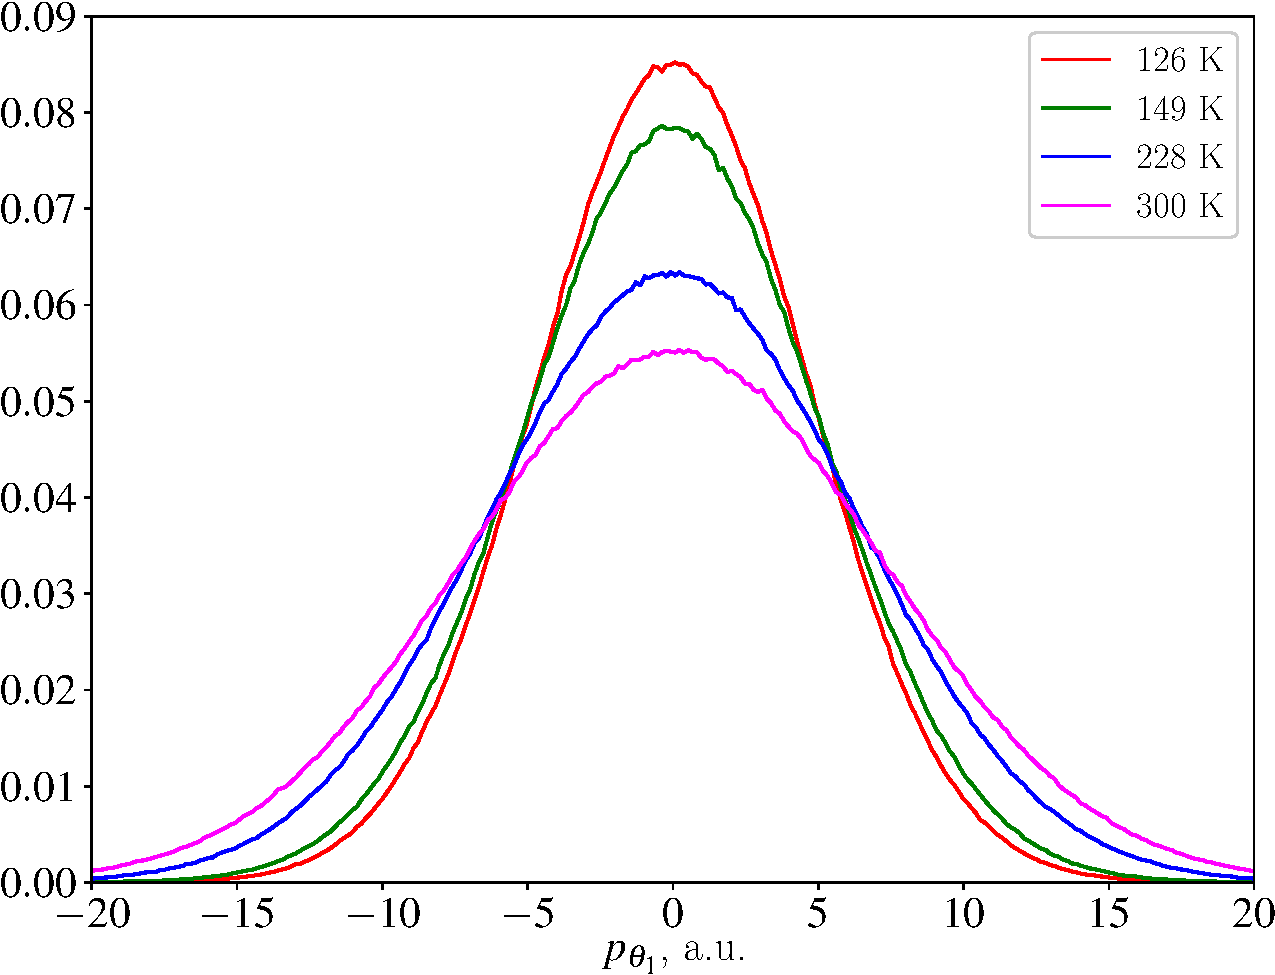
\includegraphics[width=0.75\linewidth]{./pictures/polyatom_distributions/pTheta1-crop.pdf} \\
    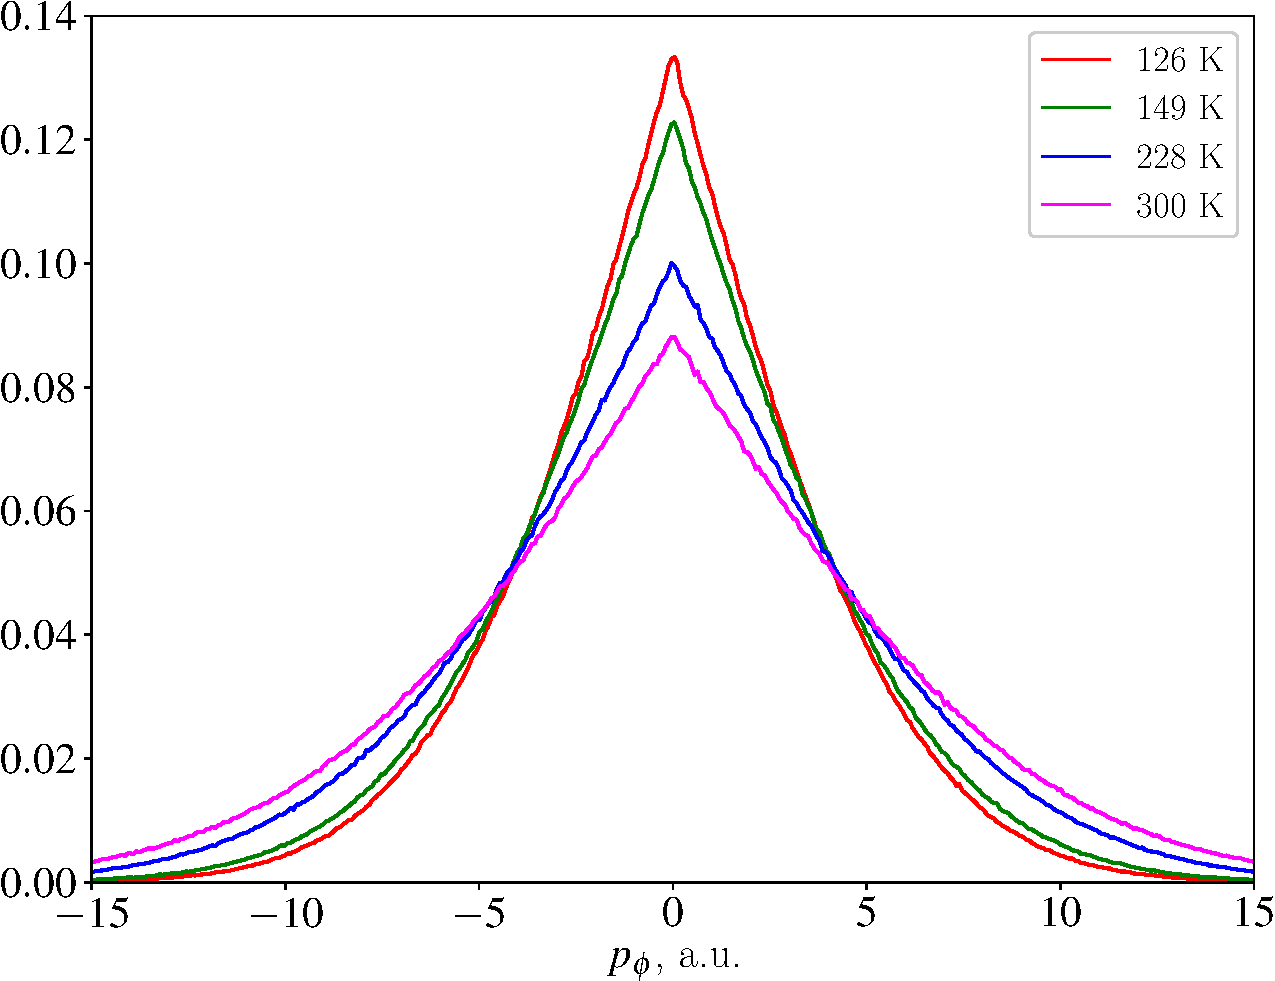
\includegraphics[width=0.75\linewidth]{./pictures/polyatom_distributions/pPhi-crop.pdf}
    \caption{Плотности распределений импульсов $p_{\theta_1}$ и $p_\varphi$ при температурах от 126К до 300К для системы N$_2-$N$_2$. Максимумы распределений убывают с увеличением температуры. Межатомное расстояние $\rfixed$ взято равным 30 $a_0$. Количество сгенерированных точек при каждой температуре -- $N = 10^7$.}
    \label{fig:polyatom-distributions}
\end{figure}

\section{Проблемы, связанные с использованием подвижной системы отсчета}

Использование подвижной системы координат вызывает некоторые вычислительные проблемы при описании динамики столкновения молекул. \par
Рассмотрим движение системы атом$-$линейная молекула в отсутствии вращения молекулярной системы относительно лабораторной системы. Пусть расстояние между атомом и линейной молекулой достаточно велико, чтобы пренебречь взаимодействием. Пусть линейная молекула претерпевает равномерное вращение относительно оси $OY$ подвижной системы. Заметим, что когда линейная молекула и атом лежат на одной оси, подвижная система координат не определена. Более того, при каждом пересечении линейной молекулой оси $OZ$ подвижной системы, изменяется направление осей $OX$ и $OY$. Это происходит, потому что угол $\theta$ определен от $0$ до $\pi$ и отсчитывается в положительную сторону направления оси $OX$. Поэтому при пересечении линейной молекулой оси $OZ$, ось $OX$ обязана изменить направление, а ось $OY$ определена так, чтобы тройка осей образовывала правую тройку. Описанная ситуация физически случается редко, однако если допустить вращение молекулярной системы, то эффект резкого поворота подвижной системы все равно будет наблюдаться. При резком вращении молекулярной системы, очевидно, существенно меняются производные эйлеровых импульсов, что вынуждает нас при численном решении системы использовать все более маленькие шаги по времени. Однако размер шагов по времени ограничен снизу, и какие-то движения системы невозможно описать в рамках двойной точности. При расчете массива траектории численное интегрирование таких траекторий обрывается, вклад таких траекторий в спектр не учитываются. Мы предполагаем, что траектории, на которых встречаются подобные вычислительные сложности, не локализованы в каких-то областях фазового пространтства и, следовательно, существенной погрешности в расчет суммарного спектрального профиля не вносят. \par
В случае пары двухатомных молекул возникает очень похожая ситуация. В этом случае плоскость подвижной системы координат $OXZ$ строится по одной из линейной молекул (будем называть ее первой) и центру массу второй линейной молекулы. Также как и в предыдущем случае, подвижная система перестает быть определена, когда линейная молекула и центр масс второй молекулы лежат на одной прямой. Рассмотрим движение в отсутствии вращения подвижной системы координат. При равномерном вращении первой молекулы вокруг оси подвижной системы $OY$, происходит обращение осей $OX$ и $OY$, когда линейная молекула пересекает ось $OZ$. Возникают те же самые вычислительные сложности, что и в случае атом$-$линейная молекула. \par
В последнем случае, засчет большего количества атомов, можно сделать преобразование, существенно снижающее количество неопределенностей системы координат. Заметим, что резкие вращения подвижной системы происходят только когда первая молекула (на которой \enquote{закреплена} плоскость подвижной системы) пересекает ось $OZ$, при этом движение второй молекулы может быть каким-угодно. Если при подходе первой молекулы к оси $OZ$ осуществить перенос плоскости подвижной системы с первой молекулы на вторую, то движение первой молекулы не приведет к резкому вращению подвижной системы. Эта замена эквивалентна перенумерации молекул. Рассмотрим преобразование гамильтоновых переменных при перенумерации молекул. \par
Преобразование углов $\theta_1$, $\theta_2$ будет происходить по следующему закону, т.к. в результате перенумерации молекул изменяет свое направление ось $OZ$ подвижной системы
\begin{gather}
    \begin{aligned}
        \theta_1^\prime &= \pi - \theta_2, \\
        \theta_2^\prime &= \pi - \theta_1.
    \end{aligned}
\end{gather}

Преобразование эйлеровых углов $\Phi^\prime$, $\Theta^\prime$ происходит точно так же, как при инверсии декартовой тройки осей, относительно которых отсчитываются сферические углы. Понятно, что преобразование эйлерова угла $\Psi$ зависит от угла $\varphi$. Точный вид преобразования был подобран исходя из соображений инвариантности лагранжиана относительно осуществляемой замены:  
\begin{gather}
    \begin{aligned}
        \Phi^\prime &= \pi + \Phi, \\
        \Theta^\prime &= \pi - \Theta, \\
        \Psi^\prime &= \pi - \Psi - \varphi.
    \end{aligned}
\end{gather}

Несложно получить преобразования скоростей при перенумерации молекул
\begin{gather}
    \begin{aligned}
        \dot{\theta}_1^\prime &= -\dot{\theta}_2, \\
        \dot{\theta}_2^\prime &= -\dot{\theta}_1, \\ 
        \dot{\Phi}^\prime &= \dot{\Phi}, \\
        \dot{\Theta}^\prime &= -\dot{\Theta}, \\
        \dot{\Psi}^\prime &= - \dot{\Psi} - \dot{\varphi}.
    \end{aligned} \label{polyatom-angles-exchange1}
\end{gather}

Получить аналогичные простые выражения для преобразования импульсов, сопряженных соотвествующим переменным, не представляется возможным, однако численно осуществить преобразование несложно. \par
Итак, пусть исходно мы имеем численные вектора обобщенных координат $\mf{q}$, сопряженных импульсов $\mf{p}$, вектор эйлеровых углов $\bUpsilon$ и эйлеровых импульсов $\pe$. Сначала рассчитаем лагранжевы скорости $\dot{\mf{q}}$ и $\dot{\boldsymbol{\Upsilon}}_e$ по соотношениям
\begin{gather}
    \begin{aligned}
        \dot{\boldsymbol{\Upsilon}}_e &= \bbW^+ \lb \bbG_{11} \bbW \pe + \bbG_{12} \mf{p} \rb, \\
        \dot{\mf{q}} &= \bbG_{12}^+ \bbW \pe + \bbG_{22} \mf{p}.
    \end{aligned}
\end{gather}

Предварительно для этого численно вычисляются матрицы $\bba$, $\bbA$, $\bbI$, и по формулам Фробениуса \eqref{polyatom-frobenius} рассчитываются матрицы $\bbG_{11}$, $\bbG_{12}$ и $\bbG_{22}$. Затем согласно полученным ранее соотношениям преобразуем лагранжевы переменные 

\begin{gather}
    \dot{\mf{q}}^\prime = 
    \begin{bmatrix}
        1 & 0 & 0 & 0 \\
        0 & 1 & 0 & 0 \\
        0 & 0 & 0 & -1 \\
        0 & 0 & -1 & 0 
    \end{bmatrix} \dot{\mf{q}}, \quad
    \dot{\boldsymbol{\Upsilon}}_e^\prime = 
    \begin{bmatrix}
        1 & 0 & 0 \\
        0 & -1 & 0 \\
        0 & 0 & -1
    \end{bmatrix}
    \dot{\boldsymbol{\Upsilon}}_e + 
    \begin{bmatrix}
        0 & 0 & 0 & 0 \\
        0 & 0 & 0 & 0 \\
        0 & -1 & 0 & 0 
    \end{bmatrix}
    \dot{\mf{q}}.
\end{gather}

После чего пересчитываем преобразованные лагранжевы переменные в гамильтоновы по соотношениям
\begin{gather}
    \begin{aligned}
        \mf{p}^\prime &= \bbA^+ \bbV \dot{\boldsymbol{\Upsilon}}_e^\prime + \bba \dot{\mf{q}}^\prime, \\
        \pe^\prime &= \bbV^+ \lb \bbI \bbV \dot{\boldsymbol{\Upsilon}}_e^\prime + \bbA \dot{\mf{q}}^\prime \rb, 
    \end{aligned}
\end{gather}

и продолжаем численное интегрирование траектории в преобразованных координатах $\mf{q}^\prime, \mf{p}^\prime, \bUpsilon^\prime$, $\pe^\prime$. \par
Понятно, что в тех случаях, когда все атомы линейных молекул выстраиваются вдоль одной линии, перенос подвижной системы не поможет. Численные расчеты показали, что доля таких траекторий имеет порядок $10^{-3} \%$. \par
В случае систем с большим количеством вращательных степеней свободы выбор подвижной системы становится шире, и, следовательно, снижается количество ситуаций, в которых невозможно определить подвижную систему. 

\section{Квантово-химические данные}

Поверхности потенциальной энергии и индуцированного дипольного момента для системы N$_2-$N$_2$ были взяты из работы \cite{karman2015}. Расчеты проводились с использованием метода связанных кластеров CCSD(T) в электронно-коррелированном базисе aug-cc-pVQZ. В полученных данных была учтена BSSE-коррекция. Дипольный момент комплекса рассчитывался методом конечного поля. Для устранения эффектов гиперполяризации в каждой геометрической конфигурации комплекса было проведено по 4 электронных расчета при разных напряженностях электрического поля. Расчеты были проведены при 29 разных взаимных ориентациях молекул и 15 разных значениях межмолекулярного расстояния. При избранных $T$-образных кофигурациях были проведены тестовые расчеты в базисе aug-cc-pV5Z. Наибольшая разница между значениями дипольного момента в двух базисах составила 0.3\%. \par
Аналитическая аппроксимация поверхности потенциальной энергии может быть выполнена в базисе сферических гармонических функций \cite{green1975} 
\begin{gather}
    V(R, \theta_1, \theta_2, \varphi) = \sum_{l_1, l_2, l} V_{l_1, l_2, l}(R) A_{l_1, l_2, l}(\theta_1, \theta_2, \varphi).
\end{gather}

Базисные функции $A_{l_1, l_2, l}(\theta_1, \theta_2, \varphi)$ являются произведениями присоединенных функций Лежандра $P^l_m(\theta)$
\begin{gather}
    A_{l_1, l_2, l}(\theta_1, \theta_2, \varphi) = \sqrt{\frac{2l+1}{4 \pi}} \Bigg[ \langle l_1 0 l_2 0 \vert l 0 \rangle P_{l_1}^0(\theta_1) P_{l_2}^0(\theta_2) + \hspace{5cm} \notag \\
    \hspace{4cm} + 2 \sum_{m} (-1)^m \langle l_1 m l_2 -m \vert l 0 \rangle P_{l_1}^m(\theta_1) P_{l_2}^m(\theta_2) \cos(m \varphi) \Bigg], 
\end{gather}
%
где через $\langle \cdots \vert \cdots \rangle$ обозначены коэффициенты Клебша-Гордона. Присоединенные функции Лежандра $P_l^m$ связаны со сферическими гармоническими функциями $Y_l^m$ соотношениями
\begin{gather}
    Y_l^m(\theta, \varphi) = P_l^m(\theta) e^{i m \varphi}.
\end{gather}

Вследствие того, что обе молекулы являются гомоядерными, оба квантовых числа $l_1$ и $l_2$ принимают четные значения. \par
Коэффициенты разложения по угловому базису были найдены авторами методом наименьших квадратов. Максимальные значения квантовых угловых чисел были взяты равными $l_1^\text{max} = l_2^\text{max} = 8$.  Радиальная зависимость коэффициентов углового базиса была аппроксимирована нами при помощи сплайнов.  \par
Разложение дипольного момента $\bs{\mu}$ 
\begin{gather}
    \bs{\mu} = \lc
    \begin{aligned}
        \mu_x &= \frac{\mu^{-1} - \mu^{+1}}{\sqrt{2}} \\
        \mu_y &= \frac{\mu^{+1} - \mu^{-1}}{i \sqrt{2}} \\
        \mu_z &= \mu^0
    \end{aligned}
    \right.
\end{gather}
%
часто записывается в угловых координатах, определенных в лабораторной системе координат. Компоненты $\mu^{0, \pm 1}$ могут быть разложены в базисе сферических функций согласно следующим формулам \cite{hartmann2011} 
\begin{gather}
    \mu^n (n = 0, \pm 1) = \frac{( 4 \pi )^{3/2}}{\sqrt{3}} \sum_{l_1, l_2, \Lambda, l} A_{l_1, l_2, \Lambda, l}(R) \sum_{m_\Lambda, m, m_1, m_2} (-1)^{l_1 + l_2 + m_\Lambda + \Lambda + l + n} \sqrt{3 (2\Lambda + 1)} \times \notag \\
    \times
    \begin{pmatrix}
        \Lambda & l & 1 \\ m_\Lambda & m & -n 
    \end{pmatrix}
    \begin{pmatrix}
        l_1 & l_2 & \Lambda \\
        m_1 & m_2 & -m_\Lambda
    \end{pmatrix}
    Y_{l_1}^{m_1}(\theta_1, \varphi_1) Y_{l_2}^{m_2}(\theta_2, \varphi_2) Y_l^m(\theta, \varphi), \label{dipole-expansion} 
\end{gather}
%
где через $(:::)$ обозначены 3j-символы Вигнера. Наборы углов $(\theta_1, \varphi_1)$, $(\theta_2, \varphi_2)$ и $(\theta, \varphi)$ описывают относительную ориентацию первой, второй и межмолекулярной оси, соответственно. Разложение \eqref{dipole-expansion} следует преобразовать к угловым координатам молекулярной системы координат, детально эти преобразования описывать не будем. \par
Коэффициенты разложения по угловому базису также были найдены методом наименьших квадратов, здесь углового базиса был ограничен максимальными значениями квантовых угловых чисел $l_1^\text{max} = l_2^\text{max} = 6$. Радиальная зависимость коэффициентов углового базиса также была аппроксимирована при помощи сплайнов. \par
Глобальный минимум поверхности потенциальной энергии достигается в скошенной конфигурации; глубина потенциальной ямы составляет около 100 см$^{-1}$ (рис. \ref{fig:n2n2-potential-curves}). Близко к глобальному минимуму расположен минимум в $T$-образной конфигурации, которая обладает наибольшим дипольным моментом. Скошенная конфигурация, являясь высокосимметричной, не обладает дипольным моментом. 

\begin{figure}[H]
    \centering
    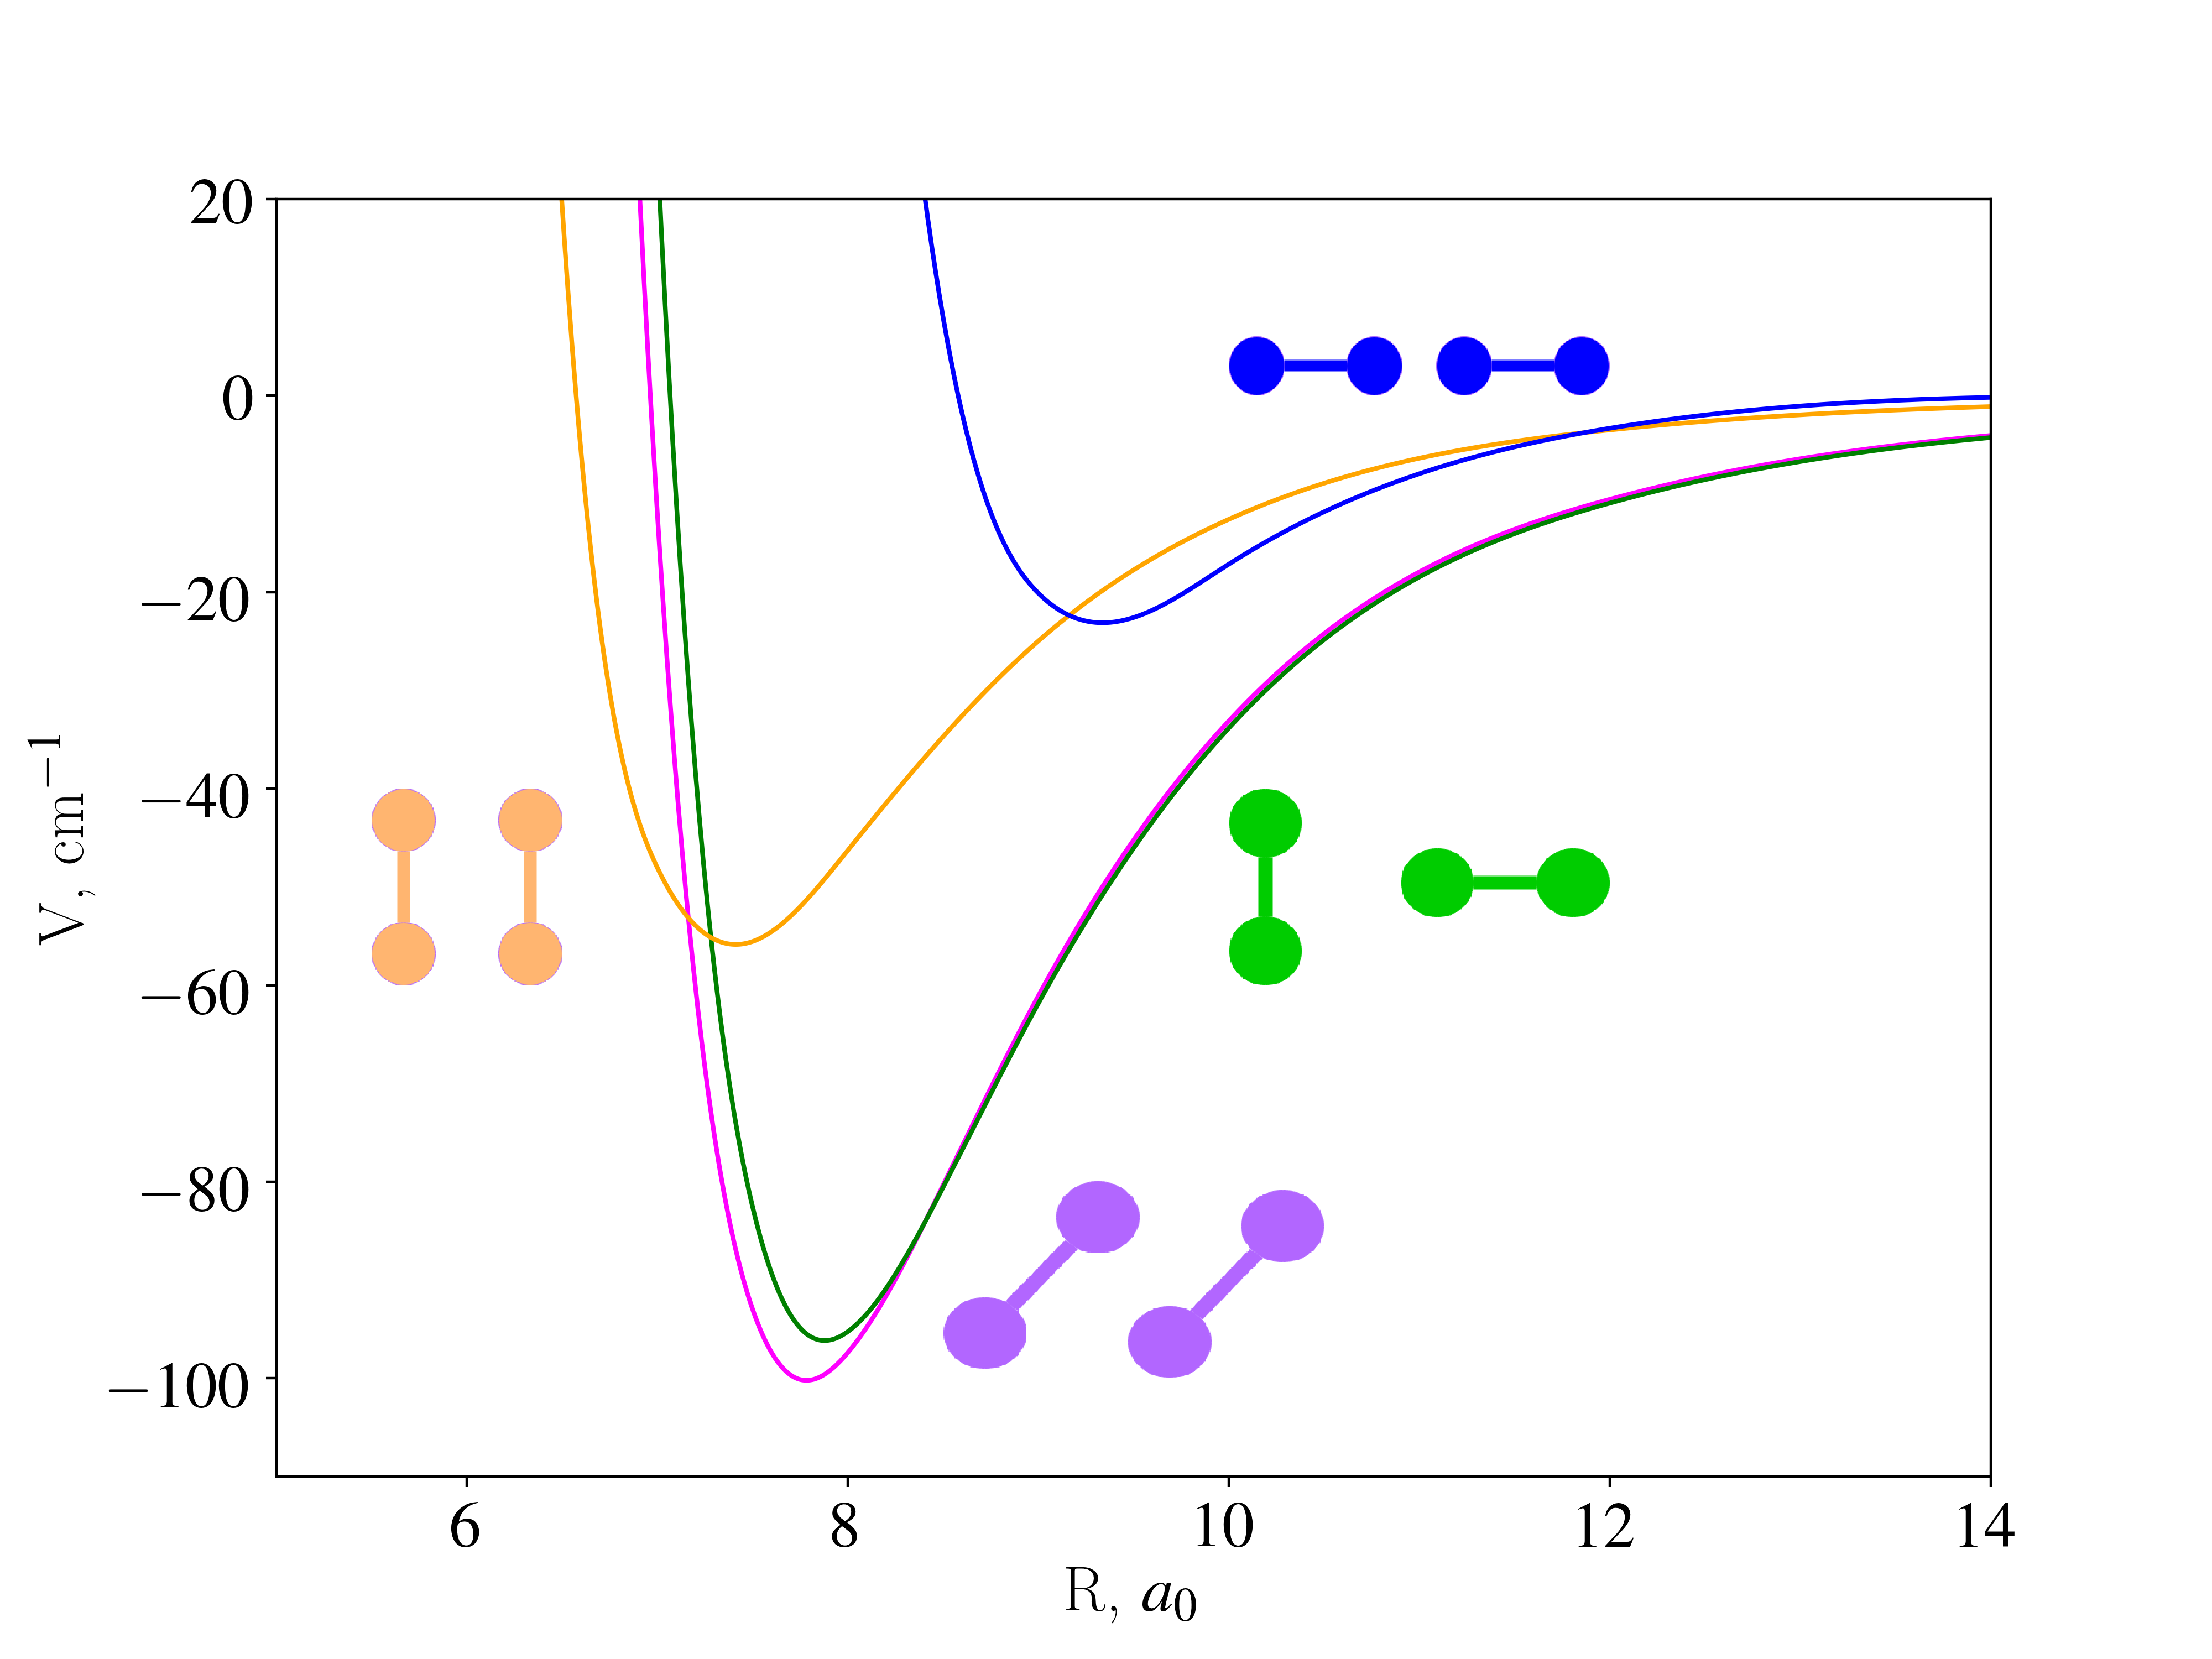
\includegraphics[width=0.75\linewidth]{./pictures/n2n2_potential.png}
    \caption{Радиальные зависимости потенциальной энергии системы N$_2-$N$_2$ в нескольких угловых конфигурациях}
    \label{fig:n2n2-potential-curves}
\end{figure}

Поверхности потенциальной энергии и индуцированного дипольного момента для системы CO$_2-$Ar были рассчитаны Ю. Калугиной. Для расчетов использовался метод связанных кластеров CCSD(T), являющийся золотым стандартом в этом классе задач. При расчете обеих поверхностях использовался электронно-коррелированный базис aug-cc-pVTZ, дополненный связевыми функциями. В полученных данных была скорректирована BSSE-ошибка. \par
Аналитическая аппроксимация \textit{ab initio} данных была выполнена в базисе полиномов Лежандра
\begin{gather}
    V(R, \theta) = \sum_{\lambda = 0}^{\lambda^\text{max}} V_\lambda(R) P_\lambda(\cos \theta). \label{co2-ar-expansion}
\end{gather}

В силу симметричности молекулы CO$_2$ в разложении \eqref{co2-ar-expansion} присутствуют только четные $\lambda$. Максимальное значение квантового числа $\lambda$ было взято равным $\lambda^\text{max} = 10$. Радиальные функции $V_\lambda(R)$ были описаны сплайнами на средних расстояниях, экспонентой -- на малых расстояниях и полиномиальными функциями -- при больших расстояниях. \par
Аналитическое представление поверхности дипольного момента может быть выполнено в базисе присоедиенных функций Лежандра. При погружении системы в плоскость подвижной системы координат $OXZ$, $y$-компонента дипольного момента константно равна нулю, а $x$- и $z$-компоненты могут быть разложены в ряды \cite{meyer1986_h2he}
\begin{gather}
    \mu_x = \sum_{\lambda = 1}^{\lambda^\text{max}} \alpha_\lambda(R) P_\lambda^1(\cos \theta), \quad \mu_z = \sum_{\lambda_1}^{\lambda^\text{max}} \beta_\lambda(R) P_\lambda^0(\cos \theta).
\end{gather}

\begin{figure}[H]
    \centering
    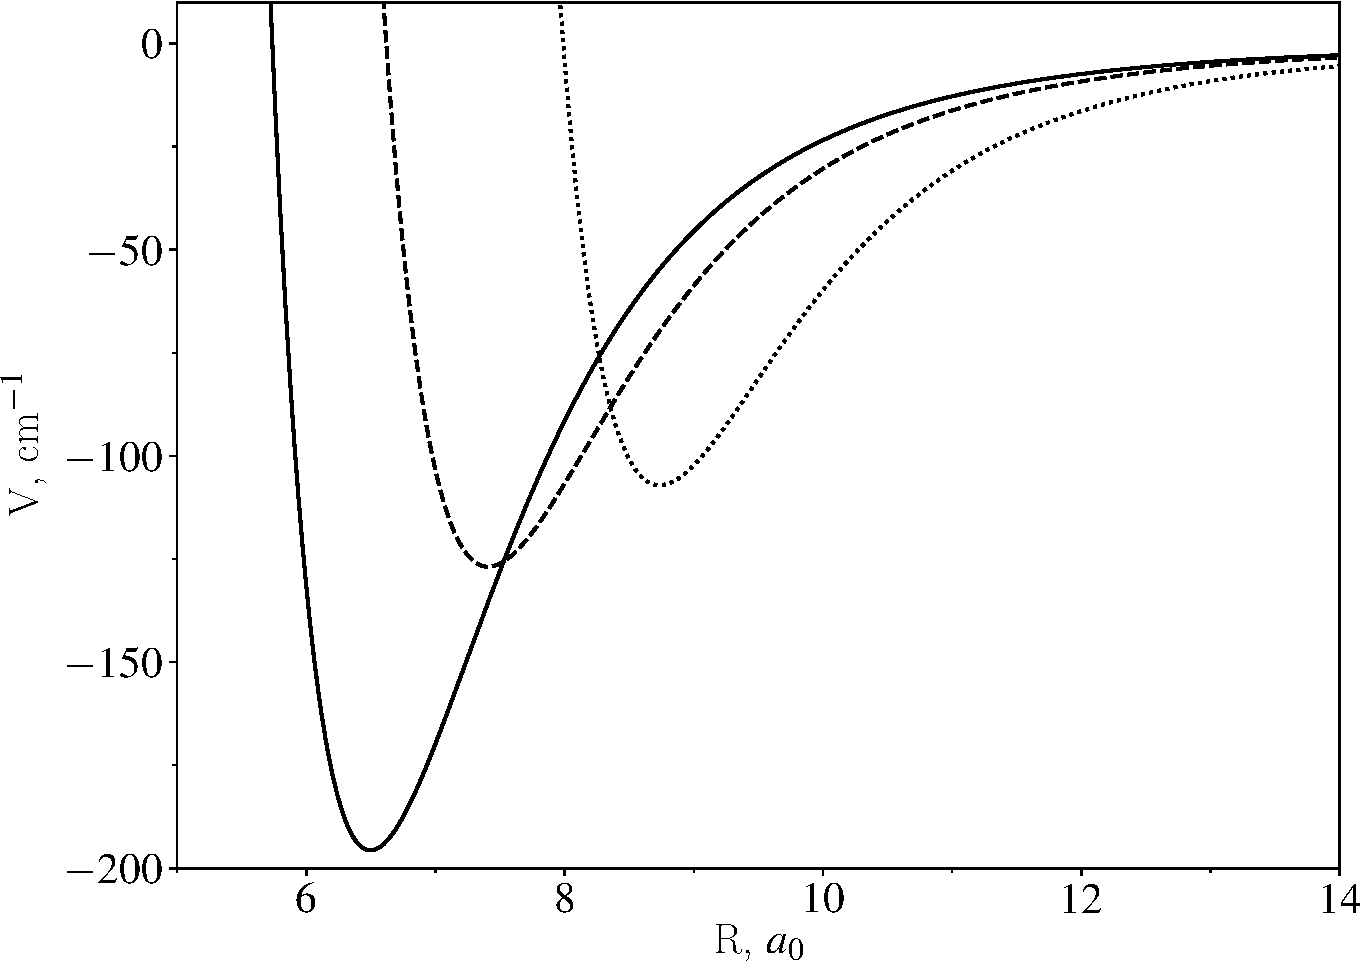
\includegraphics[width = 0.75\linewidth]{./pictures/co2-ar-potential-crop.pdf}
    \label{fig:co2-ar-potential}
    \caption{Сечения поверхности потенциальной энергии системы CO$_2-$Ar. Сплошной линией обозначена радиальная зависимость при $\theta = \pi/2$, пунктиром -- при $\theta = \pi/3$, точками -- при $\theta = 0$.}
\end{figure}

Глобальный минимум поверхности составляет примерно 196 см$^{-1}$ и достигается при $T$-образной конфигурации комплекса.

\section{Результаты траекторных расчетов}

Было предположено, что выражение для спектральной функции \eqref{two-atom-spectral-function4} обобщается на многомерные системы (то есть, что появление фактора $p_r/ \mu$ связано с заменой от интеграла по $dr$ к интегралу по $dt$ и не зависит от количества угловых переменных). Здесь $\mu$ обозначает приведенную массу комплекса как квазидухатомной системы:
\begin{gather}
    \mu = \frac{m_1 m_2}{m_1 + m_2},
\end{gather}
%
где $m_1$, $m_2$ -- массы первой и второй молекулы, соответственно. \par
Строго возможность применения этого перехода обоснована не была, однако результаты численных экспериментов показывают, что эта формула верна. \par
Итак, обобщение \eqref{two-atom-spectral-function4} на многомерные системы выглядит следующим образом
\begin{gather}
    V J(\omega) =  \frac{V}{4 \pi \varepsilon_0} \frac{1}{2\pi \Gamma_0}\int_0^\infty \frac{p_r}{\mu} dp_r \int \exp \lb -\frac{H}{\kb T} \rb d\mf{q}^\prime d\mf{p}^\prime d\bUpsilon d\pe \Bigg\vert \intty \bs{\mu}(t) e^{-i \omega t} dt \Bigg\vert^2, \label{polyatom-spectral-function1} 
\end{gather}
%
где $d\mf{q}^\prime$ содержит дифференциалы только угловых координат, а $d\mf{p}^\prime$ -- дифференциалы импульсов, сопряженные угловым координатам. \par
Интегрирование в \eqref{polyatom-spectral-function1} будем производить методом Монте-Карло с весовой функцией $p_\xi(\bxi) = \exp \lb - H(\bxi)/\kb T \rb / \Gamma_1$, где $\bxi = \lb p_r, \mf{p}^\prime, \bUpsilon, \pe \rb$, а $\Gamma_1$ -- нормировочный множитель, равный
\begin{gather}
    \Gamma_1 = \int_0^\infty dp_r \int \exp \lb -\frac{H}{\kb T} \rb d\mf{q}^\prime d\mf{p}^\prime d\bUpsilon d\pe.
\end{gather}

Рассмотрим выражение \eqref{polyatom-spectral-function1} как математическое ожидание квадрата преобразования Фурье на распределении $\bxi$
\begin{gather}
    VJ(\omega) = \frac{V}{4 \pi \varepsilon_0} \frac{\Gamma_1}{2 \pi \Gamma_0} \sum_{k = 1}^\infty \frac{p_r(\bxi_k)}{\mu} \Bigg\vert \intty \bs{\mu}(t; \bxi_k) e^{-i \omega t} dt \Bigg\vert^2,
\end{gather}
%
где используются те же обозначения, что и в выкладках для системы двух атомов. Несложно показать, что отношение нормировочных интегралов в общем случае будет равным
\begin{gather}
    \frac{V \Gamma_1}{2 \pi \Gamma_0} = \rfixed^2.
\end{gather}

Следовательно, итоговое выражение для спектральной функции как среднего по распределению $\bxi$ в многомерном случае выглядит таким же образом, как и для системы двух атомов:
\begin{gather}
    V J(\omega) = \frac{\rfixed^2}{4 \pi \varepsilon_0} \sum_{k = 1}^\infty \frac{p_r(\bxi_k)}{\mu} \Bigg\vert \intty \bs{\mu}(t; \bxi_k) e^{-i \omega t} dt \Bigg\vert^2. \label{polyatom-spectral-function2}
\end{gather}

\begin{figure}[H]
    \centering
    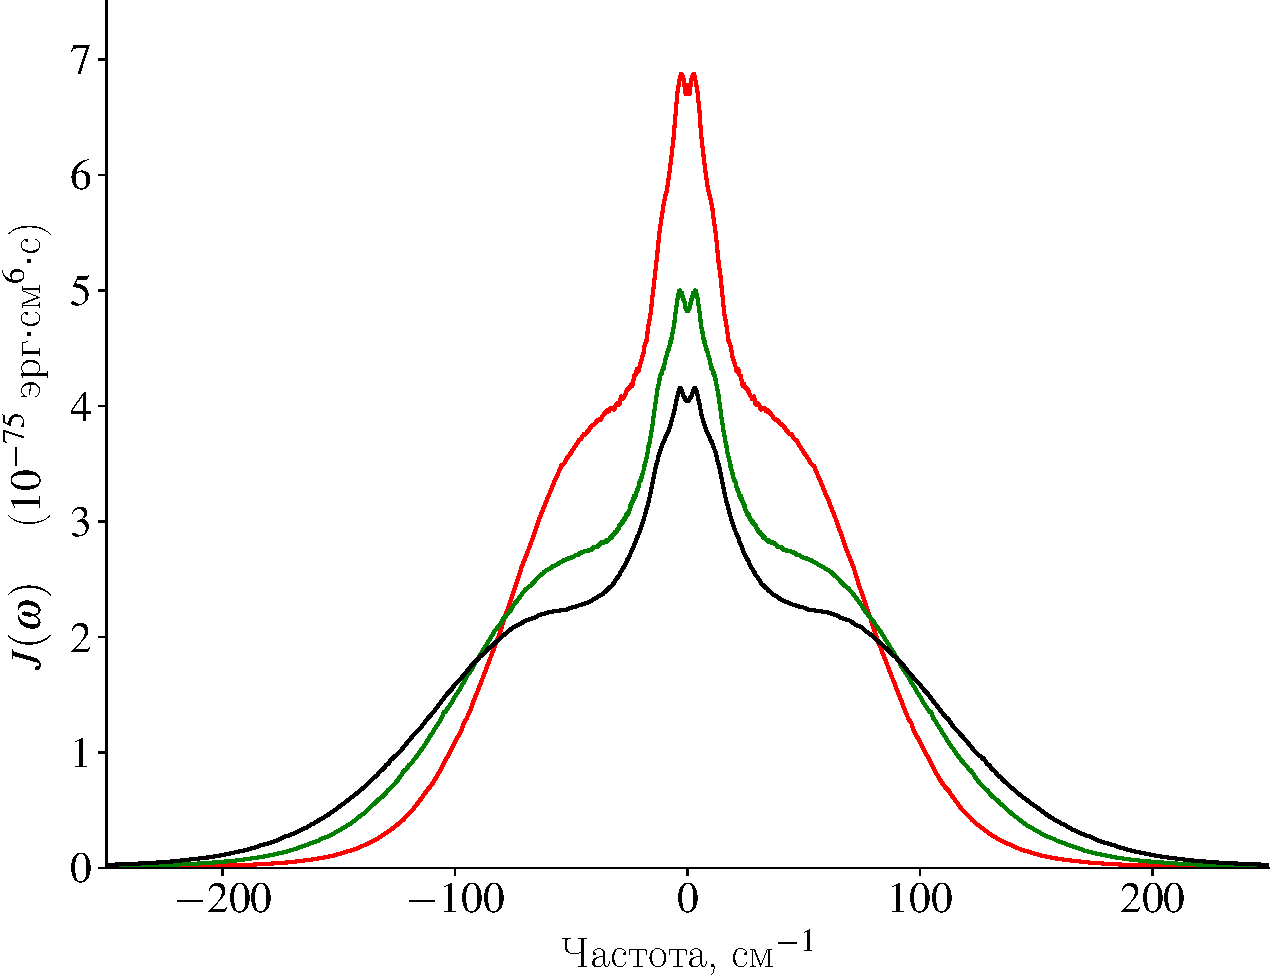
\includegraphics[width=0.7\linewidth]{./pictures/polyatom_spectra/n2n2_spectral_functions-crop.pdf}
    \caption{Классические спектральные функции системы N$_2-$N$_2$ при температурах 149К (верхняя красная кривая), 228К (средняя зеленая кривая) и 300К (нижняя черная кривая).}
    \label{fig:n2n2-spectral-functions}
\end{figure}

Для сравнения с экспериментальными данными спектральная функция, полученная по \eqref{polyatom-spectral-function2},  подвергалась процедуре десимметризации D3 \eqref{d3}. Для систем CO$_2-$Ar и N$_2-$N$_2$ влияние процедуры десимметризации достаточно велико даже при комнатной температуре, что продемонстрировано на рисунке \ref{fig:n2n2-desymmetrization}. 

\begin{figure}[H]
    \centering
    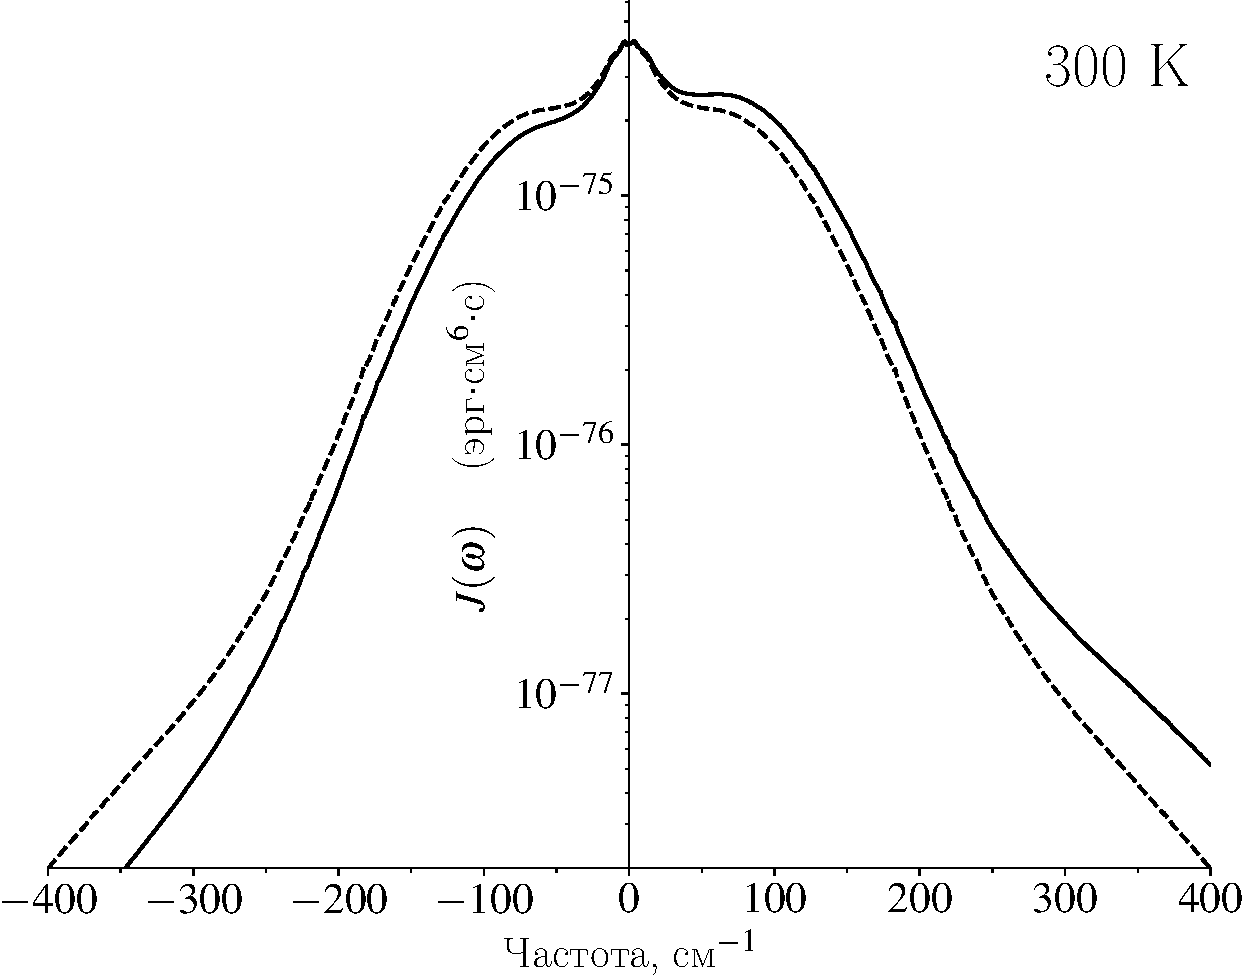
\includegraphics[width=0.49\linewidth]{./pictures/polyatom_spectra/n2n2_spectral_function_300K-crop.pdf}
    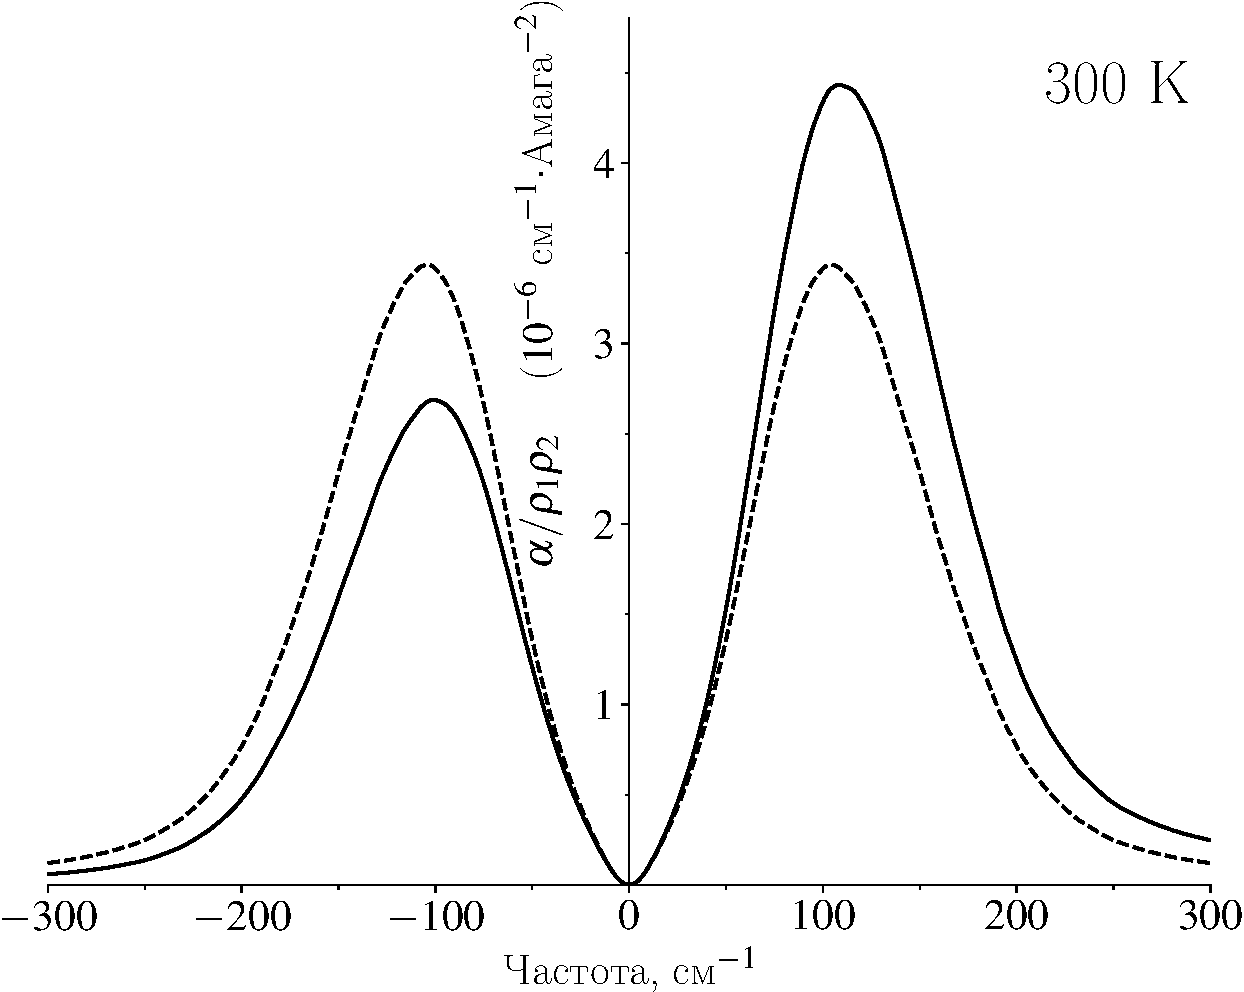
\includegraphics[width=0.49\linewidth]{./pictures/polyatom_spectra/n2n2_desymmetrization-crop.pdf}
    \caption{Влияние дессиметризации на спектральную функцию и спектральный профиль на примере спектральной функции системы N$_2-$N$_2$ при 300К. Пунктиром обозначены классические спектральные функция и профиль; сплошной линией -- полученные из классических в результате процедуры D3.}
    \label{fig:n2n2-desymmetrization}
\end{figure}

На рис. (\ref{fig:n2n2-spectra}) представлено сопоставление рассчитанных спектральных профилей системы N$_2-$N$_2$ с другими расчетными и экспериментальными данными.

\begin{figure}[H]
    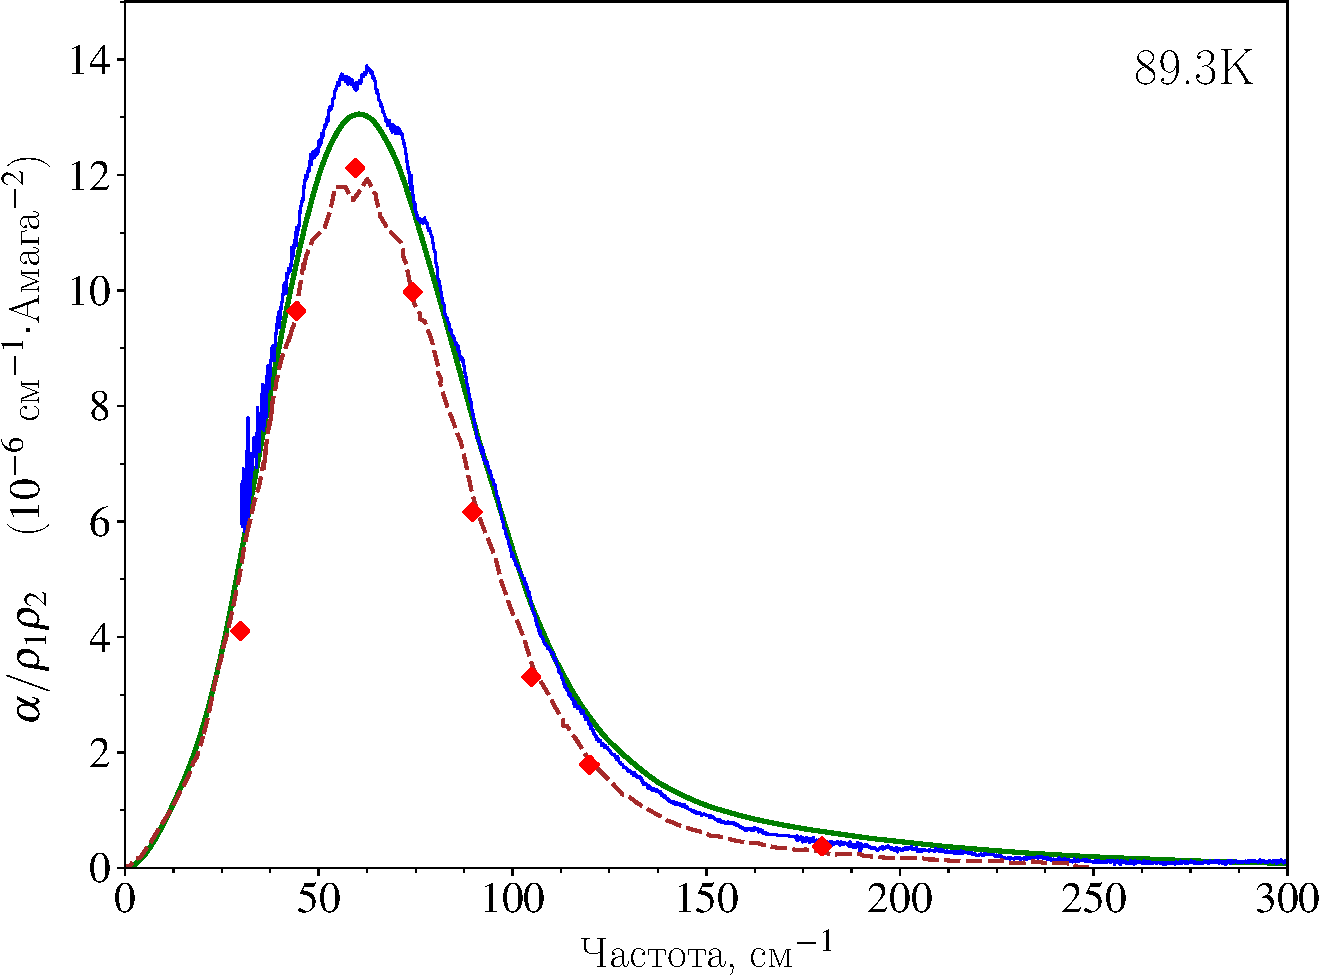
\includegraphics[width=0.49\linewidth]{./pictures/polyatom_spectra/89_3K_russian-crop.pdf} 
    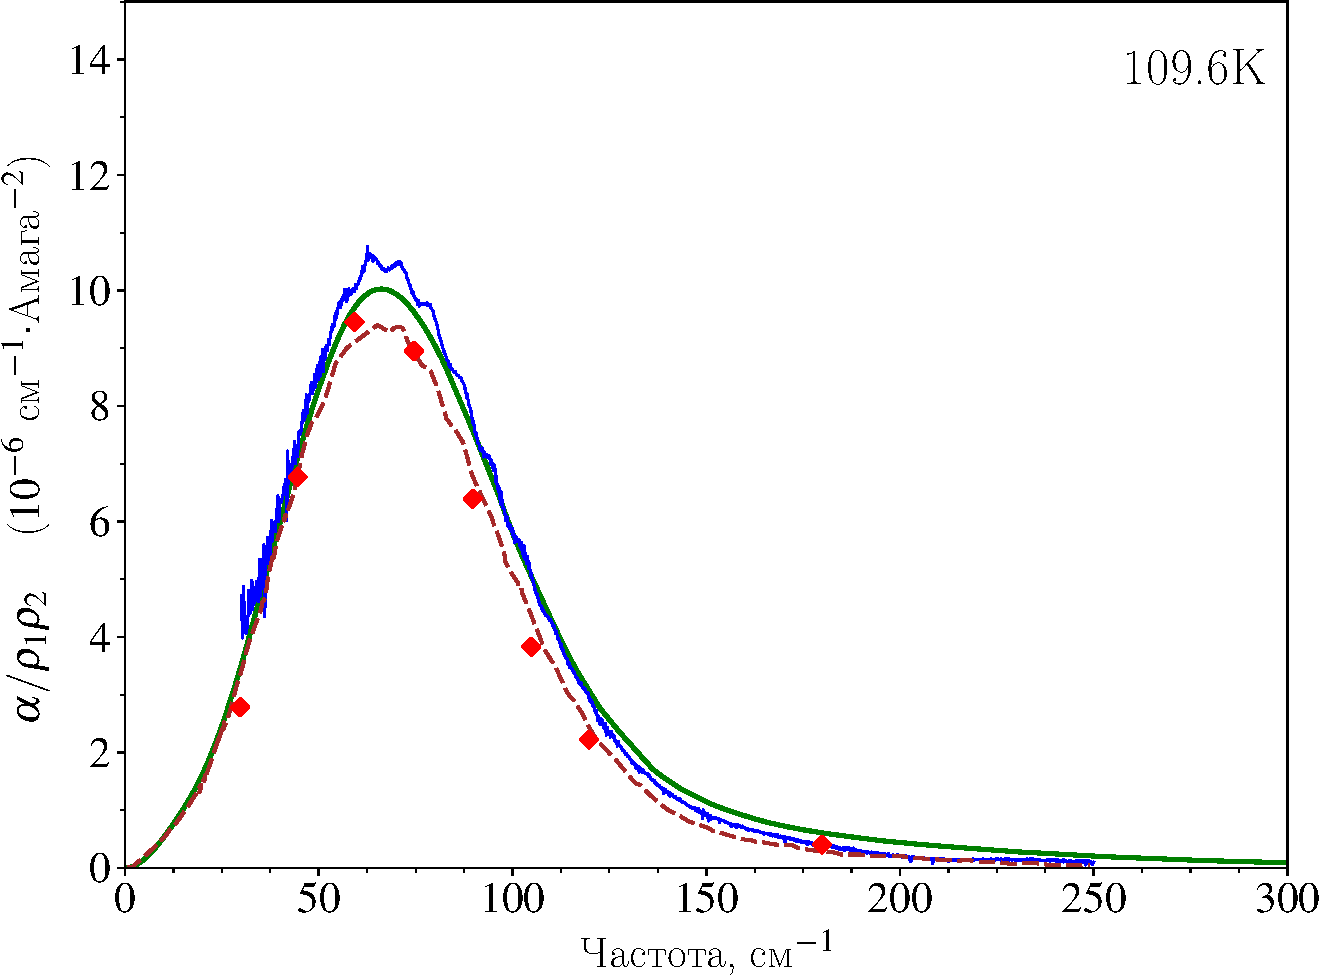
\includegraphics[width=0.49\linewidth]{./pictures/polyatom_spectra/109_6K_russian-crop.pdf} \\ 
    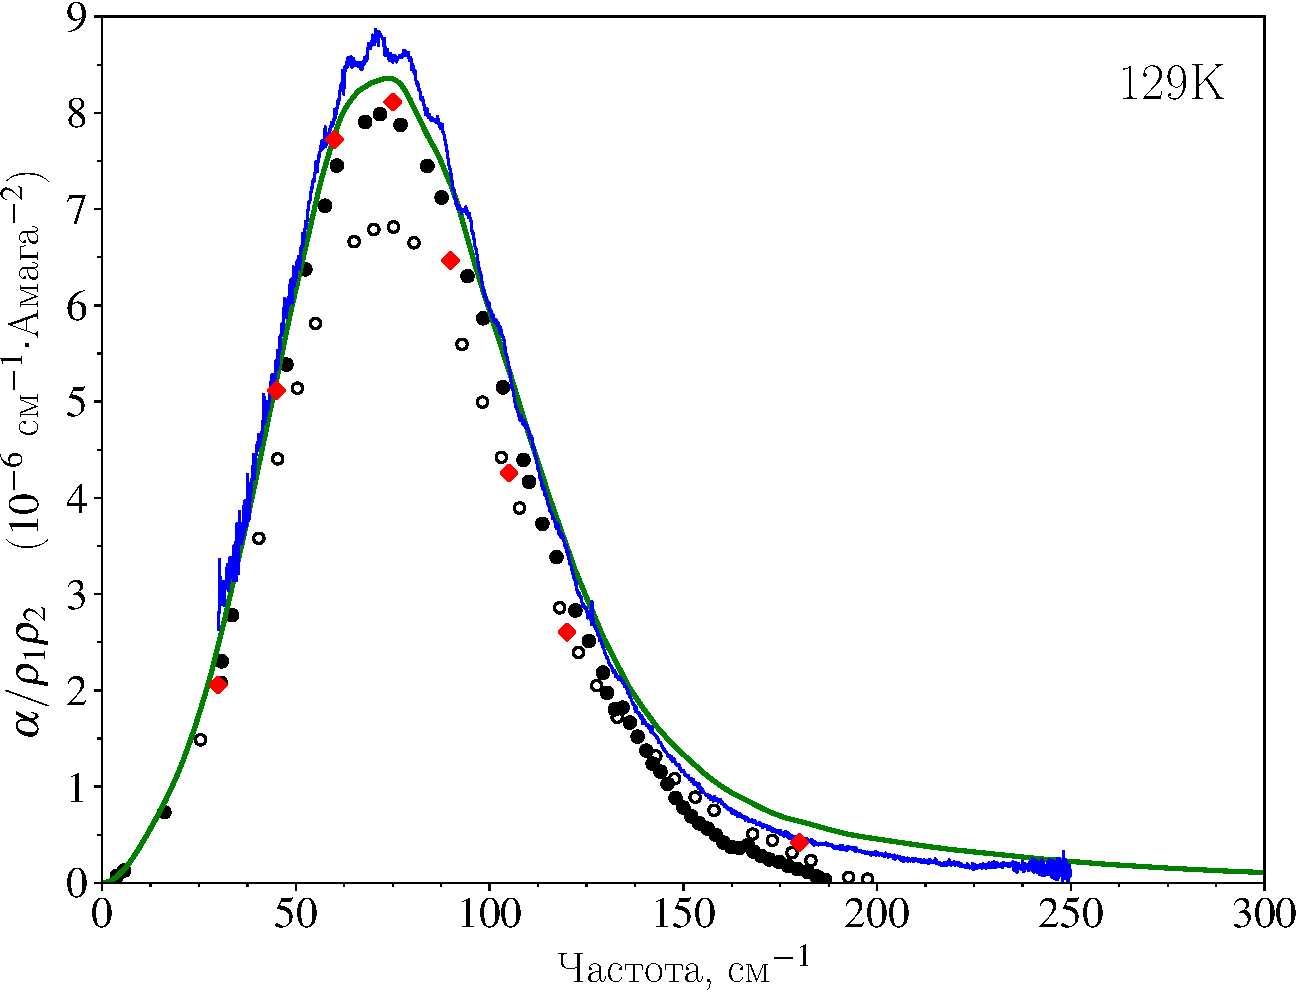
\includegraphics[width=0.49\linewidth]{./pictures/polyatom_spectra/129K_russian-crop.pdf} 
    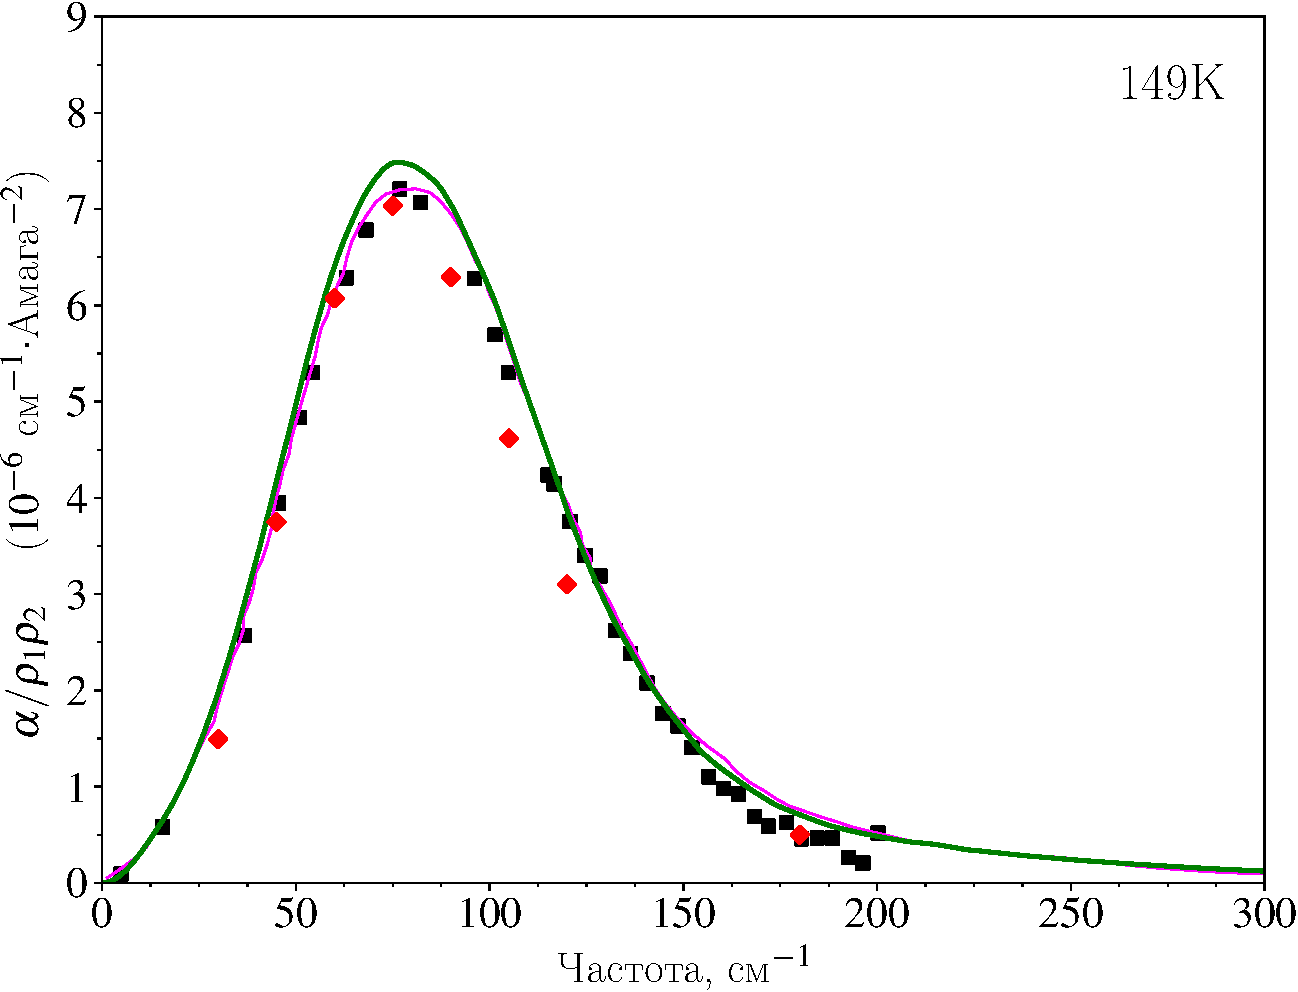
\includegraphics[width=0.49\linewidth]{./pictures/polyatom_spectra/149K_russian-crop.pdf} \\ 
    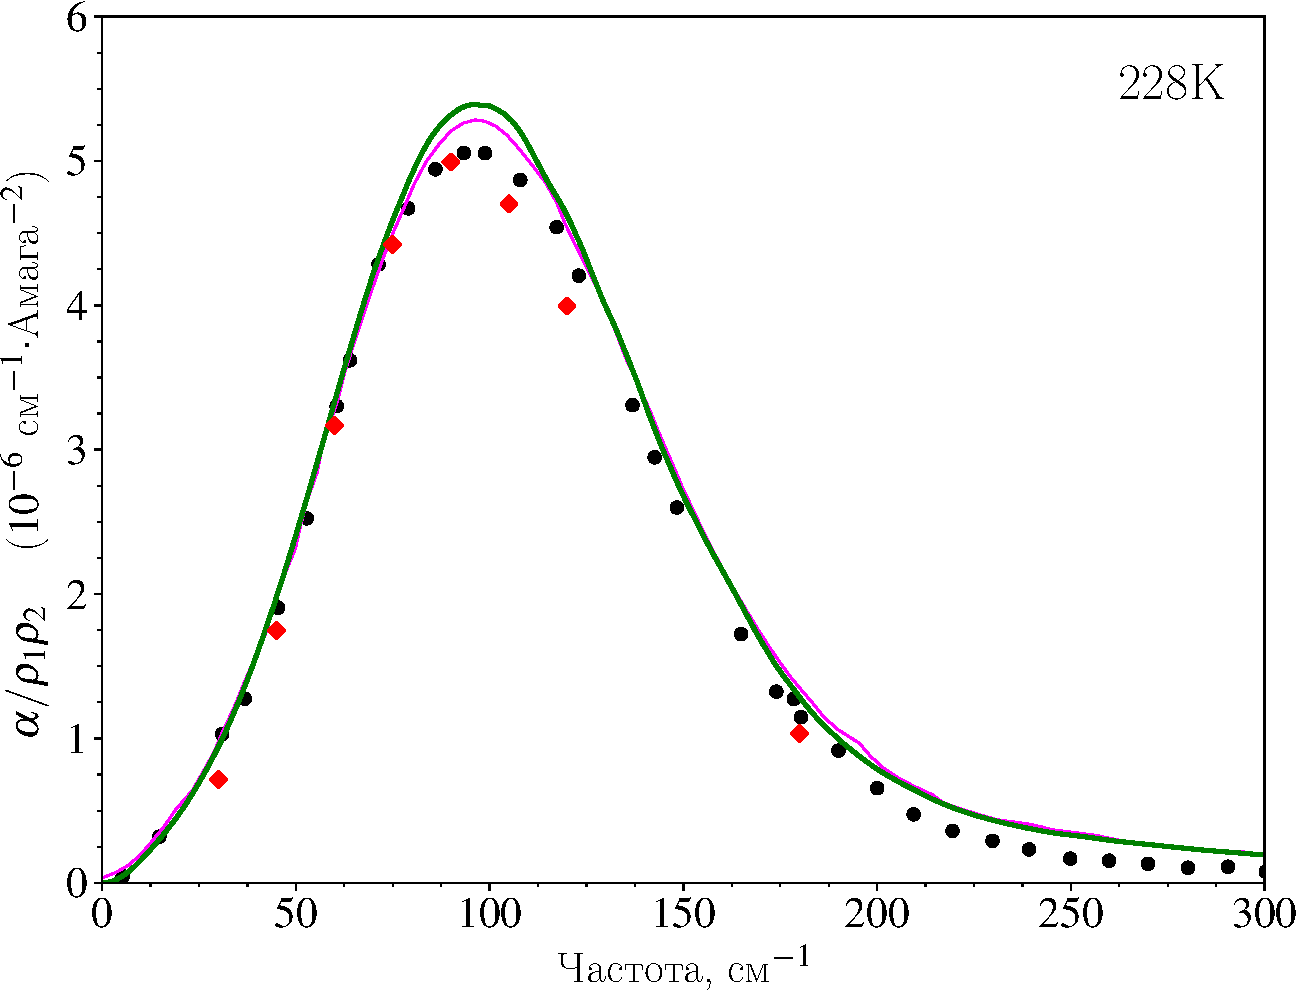
\includegraphics[width=0.49\linewidth]{./pictures/polyatom_spectra/228K_russian-crop.pdf} 
    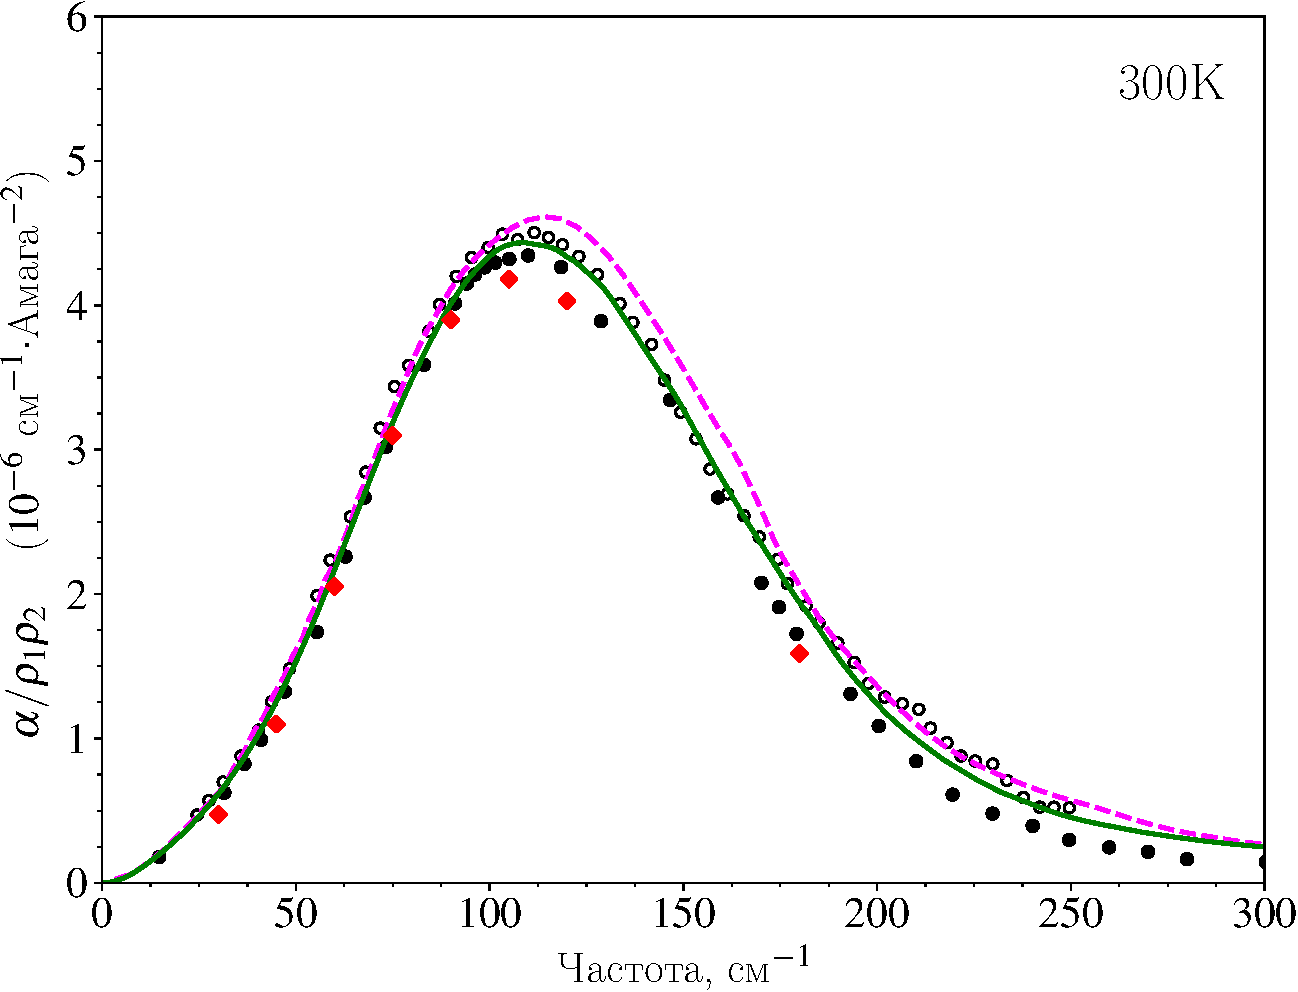
\includegraphics[width=0.49\linewidth]{./pictures/polyatom_spectra/300K_russian-crop.pdf}
    \label{fig:n2n2-spectra}
    \caption{Сопоставление рассчитанных спектральных профилей системы N$_2-$N$_2$ в области рототрансляционной полосы с расчетными и экспериментальными данными при температурах 89.3K, 109.6K, 129K, 149K, 228K и 300K. Рассчитанные в этой работе профили обозначены жирной зеленой линией. Красными ромбами обозначены интеполированные результаты квантовомеханического расчета \cite{karman2015}. Сиреневой пунктирной линией при температурах 149K, 228K и 300K обозначены результаты молекулярно-динамического расчета \cite{bussery2014}. Тонкой синей линии при температурах 89.3K, 109.6K и 129К обозначены экспериментальные данные из \cite{karman2019}. Коричневой пунктирной линией при температурах 89.3К и 109.6К обозначены результаты изотропного квантово-механического расчета \cite{borysow1986}. Черными кружками при температурах 129K, 228K и 300K обозначены экспериментальные данные из \cite{stone1984}, пустыми кружками при температурах 129К и 300К -- из \cite{buontempo1975}; черными квадратами при температуре 149К -- из \cite{dagg1985}. }  
\end{figure}

Траекторные расчеты производились с теми же поверхностями потенциальной энергии и индуцированного дипольного момента, что и квантово-механические расчеты в \cite{karman2015}. Как уже отмечалось при рассмотрении двухатомных спектров, процедура десимметризации D3 переоценивает квантовую спектральную функцию, поэтому расхождения в области крыла спектра могут быть объяснены неточностью десимметризации. Авторы \cite{karman2015} отмечают, что недостаточное количество \textit{ab initio} точек могло вызывать погрешности в коэффициентах сферических функций, используемых для аппроксимации данных. Вклад связанных состояний в интегральную интенсивность при рассматриваемых температур достаточно невелик
\begin{gather}
    \begin{aligned}
        89.3K  &: \quad M_0^\text{bound} / M_0^\text{full} = 5.5\%, \quad M_2^\text{bound} / M_2^\text{full} = 1.5\%, \\
        109.6K &: \quad M_0^\text{bound} / M_0^\text{full} = 3.0\%, \quad M_2^\text{bound} / M_2^\text{full} = 0.6\%, \\
        129.0K &: \quad M_0^\text{bound} / M_0^\text{full} = 1.8\%, \quad M_2^\text{bound} / M_2^\text{full} = 0.3\%. 
    \end{aligned}
\end{gather}
При более высоких температурах интегральный вклад связанных состояний становится пренебрежимо малым. Тем не менее, несмотря на пренебрежение связанными состояниями в нашем расчете, полученные нами профили по интенсивности более точно согласаются с экспериментальными данными \cite{karman2019}, чем результаты \cite{karman2015} и \cite{borysow1986}. \par
Авторы \cite{karman2019} оценивают погрешность экспериментальных измерений при более низких температурах в 3\% в области максимума спектрального профиля. Для экспериментальных данных \cite{stone1984}, \cite{buontempo1975}, \cite{dagg1985} принято оценивать погрешность в 10\% в области максимума поглощения. \par
Спектральные профили при низких температурах обладают двумя особенностями на фоне широкого континуального спектра -- в области малых частот наблюдается набор резких пиков и в области максимума спектра наблюдается волнистая структура, часто называемая риплами. Ранее эти особенности были обнаружены для спектра в области фундаментального перехода азота в системах N$_2-$N$_2$ и N$_2-$Ar \cite{mckellar1988}, в рототрансляционной области для системы N$_2-$N$_2$ наблюдались впервые в работе \cite{wishnow1996}. Авторы \cite{mckellar1988}, ссылаясь на теоретический анализ структуры риплов, наблюдаемых в системе N$_2-$Ar \cite{brocks1988}, связывают их с проявлениями связанных и метастабильных состояний. Отметим, что результаты изотропного квантового расчета \cite{borysow1986} обладают волнистой структурой в области максимума. \par 
Контроль сходимости расчета спектров производился при помощи спектральных моментов. Если на всех стадиях расчета не вносится систематических ошибок, то с увеличением количества траекторий спектральные моменты траекторного спектра должны совпасть со спектральными моментами, посчитанными по области фазового пространства, соответствующей свободным и метастабильным состояниям. Каждый из представленных на рис. (\ref{fig:n2n2-spectra}) получен в результате усреднения по 2.000.000 траекториям. Спектральные моменты посчитаны по области фазового пространства с энергией комплекса больше нуля при помощи адаптивного метода Монте-Карло \cite{hep}. Сравнение спектральных моментов представлено в таблице (\ref{table:n2n2-moments}).

\begin{table}[H]
    \begin{tabular}{c >{\centering}p{6cm} >{\centering}p{6cm} >{\centering}p{3cm}}
        \toprule
        $T$, K & Спектральные моменты $M_0$ (см$^{-1} \cdot$Амага$^{-2}$) и $M_2$ (см$^{-3} \cdot$Амага$^{-2}$) по фазовому пространству & Спектральные моменты $M_0$ (см$^{-1} \cdot$Амага$^{-2}$) и $M_2$ (см$^{-3} \cdot$Амага$^{-2}$) по траекторному спектру & Отклонение \tabularnewline
        \midrule
        \multirow{2}{*}{$89.3$}  & $5.487\cdot 10^{-5}$ & $5.493 \cdot 10^{-5}$ & $+0.1$ \%  \tabularnewline
                                 & $1.068\cdot 10^{-1}$ & $1.087 \cdot 10^{-1}$ & $+1.7$ \%  \tabularnewline
        \midrule
        \multirow{2}{*}{$109.6$} & $4.817\cdot 10^{-5}$ & $4.826 \cdot 10^{-5}$ & $+0.2$ \%  \tabularnewline
                                 & $1.137\cdot 10^{-1}$ & $1.144 \cdot 10^{-1}$ & $-0.7$ \%  \tabularnewline
        \midrule
        \multirow{2}{*}{$129.0$} & $4.444\cdot 10^{-5}$ & $4.414 \cdot 10^{-5}$ & $+0.7$ \%  \tabularnewline
                                 & $1.227\cdot 10^{-1}$ & $1.232 \cdot 10^{-1}$ & $-0.4$ \%  \tabularnewline
        \midrule
        \multirow{2}{*}{$149.0$} & $4.178\cdot 10^{-5}$ & $4.271 \cdot 10^{-5}$ & $+2.2$ \%  \tabularnewline
                                 & $1.332\cdot 10^{-1}$ & $1.357 \cdot 10^{-1}$ & $+1.9$ \%  \tabularnewline
        \midrule
        \multirow{2}{*}{$228.3$} & $3.756\cdot 10^{-5}$ & $3.768 \cdot 10^{-5}$ & $+0.3$ \%  \tabularnewline
                                 & $1.848\cdot 10^{-1}$ & $1.859 \cdot 10^{-1}$ & $+0.6$ \%  \tabularnewline
        \midrule
        \multirow{2}{*}{$300.0$} & $3.650\cdot 10^{-5}$ & $3.576 \cdot 10^{-5}$ & $-2.0$ \%  \tabularnewline
                                 & $2.389\cdot 10^{-1}$ & $2.339 \cdot 10^{-1}$ & $-2.1$ \%  \tabularnewline
        \bottomrule
    \end{tabular}
    \caption{Сравнение спектральных моментов, рассчитанных по фазовому пространству, с моментами по траекторным спектрам системы N$_2-$N$_2$}
    \label{table:n2n2-moments}
\end{table}

На рис. \ref{fig:co2ar-spectra} приведено сравнение рассчитанных спектров для системы CO$_2-$Ar с экспериментальными данным из \cite{tonkov1995}. При обеих температурах расхождение в максимуме спектрального профиля с экспериментальными данными составляет около 10-12\%, что попадает в интервал погрешности 10\%, который часто приписывается экспериментальным данным.
Отметим, что при экспериментальном изучении газовой смеси CO$_2-$Ar в изучаемом диапазоне часто поглощают как молекулярные пары CO$_2-$Ar, так и пары CO$_2-$CO$_2$. Максимум поглощения комплекса CO$_2-$CO$_2$ при обеих рассматриваемых температурах находится очень близок к максимуму поглощения комплекса CO$_2-$Ar \cite{gruszka1997}. Следовательно, наблюдаемое расхождение может быть связано и с погрешностями, связанными с определением поглощения комплекса CO$_2-$CO$_2$.

\begin{figure}[H]
    \centering
    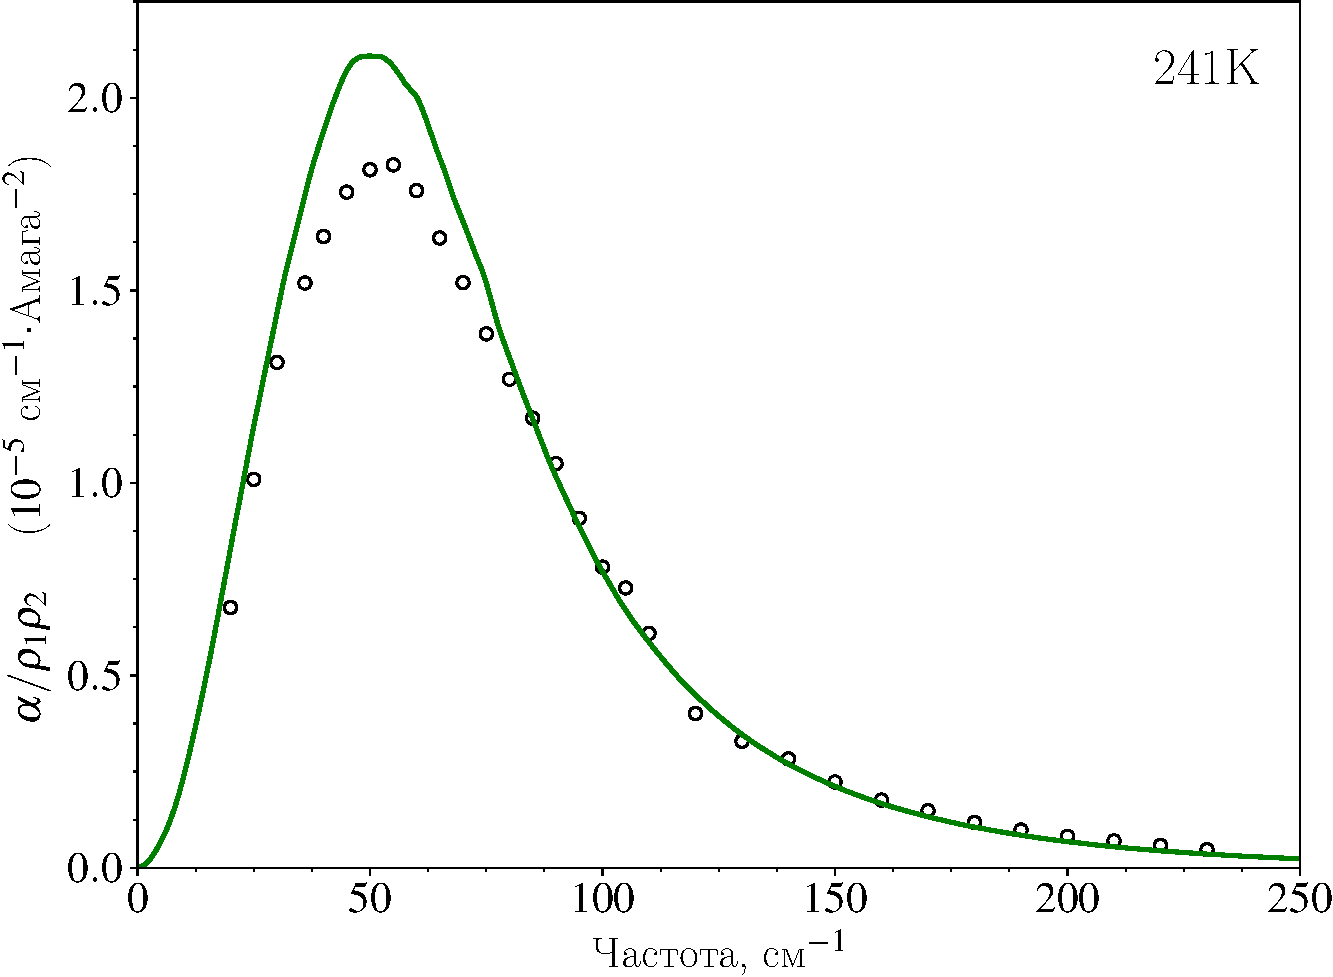
\includegraphics[width=0.49\linewidth]{./pictures/polyatom_spectra/co2_ar/241K_russian-crop.pdf}
    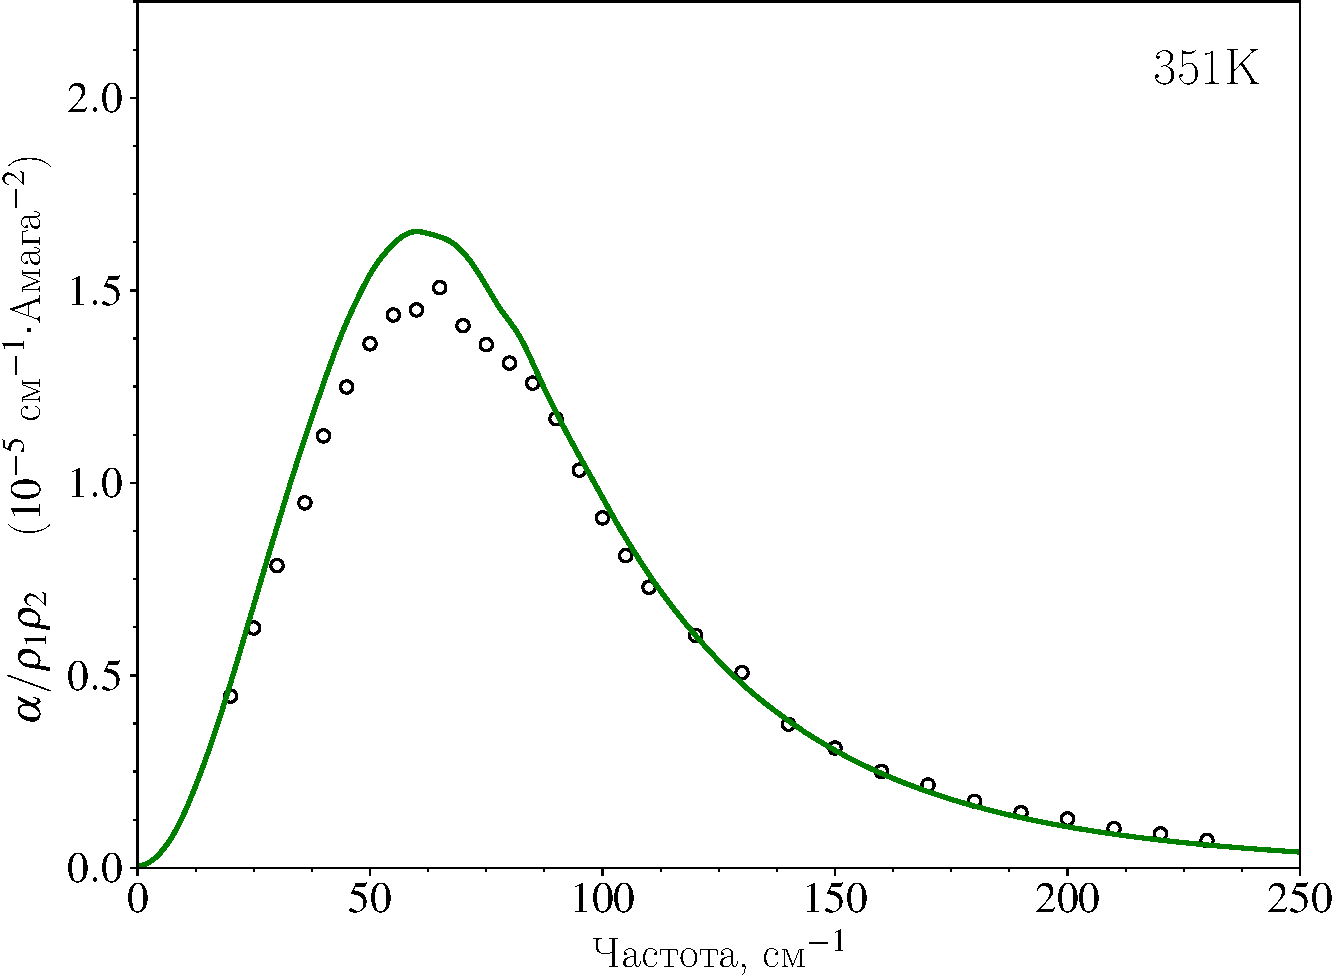
\includegraphics[width=0.49\linewidth]{./pictures/polyatom_spectra/co2_ar/351K_russian-crop.pdf}
    \label{fig:co2ar-spectra}
    \caption{Сопоставление рассчитанных спектральных профилей системы CO$_2-$Ar в области рототрансляционной полосы с экспериментальными данными из \cite{tonkov1995} при температурах 241K и 351K.}
\end{figure}

Каждый из спектров, представленных на рис. (\ref{fig:co2ar-spectra}) получен в результате усреднения по 1.000.000 траекторий. Данные о сходимости расчета по спектральным моментам представлены в таблице (\ref{table:co2ar-moments}). 

\begin{table}[H]
    \begin{tabular}{c >{\centering}p{6cm} >{\centering}p{6cm} >{\centering}p{3cm}}
        \toprule
        $T$, K & Спектральные моменты $M_0$ (см$^{-1} \cdot$Амага$^{-2}$) и $M_2$ (см$^{-3} \cdot$Амага$^{-2}$) по фазовому пространству & Спектральные моменты $M_0$ (см$^{-1} \cdot$Амага$^{-2}$) и $M_2$ (см$^{-3} \cdot$Амага$^{-2}$) по траекторному спектру & Отклонение \tabularnewline
        \midrule
        \multirow{2}{*}{$241.0$} & $3.851 \cdot 10^{-4}$ & $3.730 \cdot 10^{-4}$ & $-3.1$ \%  \tabularnewline
                                 & $5.502 \cdot 10^{-1}$ & $5.417 \cdot 10^{-1}$ & $-1.5$ \%  \tabularnewline
        \midrule
        \multirow{2}{*}{$351.0$} & $3.638 \cdot 10^{-4}$ & $3.493 \cdot 10^{-4}$ & $-0.8$ \%  \tabularnewline
                                 & $7.229 \cdot 10^{-1}$ & $7.276 \cdot 10^{-1}$ & $+0.4$ \%  \tabularnewline
        \bottomrule
    \end{tabular}
    \caption{Сравнение спектральных моментов, рассчитанных по фазовому пространству, с моментами по траекторным спектрам системы CO$_2-$Ar}
    \label{table:co2ar-moments}
\end{table}


\begin{subappendices}
    \section{Вектор углового момента в подвижной системе отсчета} \label{appendix:angular-momentum-body-fixed}

    Рассмотрим производную кинетической энергии в лагранжевой форме $\Tl$ по вектору угловой скорости $\bOmega$, компонентны которого выражены в подвижной системе отсчета. Продифференцировав выражение \eqref{body-fixed-lagrange-energy} по вектору угловой скорости, получаем 
    \begin{gather}
        \frac{\partial \Tl}{\partial \bOmega} = \bbA \dot{\mf{q}} + \bbI \bOmega. \label{appendix-angular-momentum1}
    \end{gather}

    Несложно показать, что вектор углового момента $\mf{j}$ в лабораторной системе отсчета может быть записан через векторы Якоби как
    \begin{gather}
        \mf{j} = \sum_{i = 1}^{N - 1} \mu_i \lsq \bs{\rho}_i \times \dot{\bs{\rho}}_i \rsq. \label{appendix-angular-momentum-jacobi-vectors}
    \end{gather}

    Выразим производная вектора $\bs{\rho}_i$ в лабораторной системе координат через производную в подвижной системе координат \cite{goldstein}
    \begin{gather}
        \dot{\bs{\rho}}_i = \bbS \lb \dot{\mf{R}}_i + \lsq \bs{\Omega} \times \mf{R}_i \rsq \rb. \label{appendix-jacobi-vector-derivative} 
    \end{gather}

    Подставив выражение \eqref{appendix-jacobi-vector-derivative} в выражение углового момента \eqref{appendix-angular-momentum-jacobi-vectors} и осуществив несложные алгебраические преобразования, приходим к 
    \begin{gather}
        \mf{j} = \sum_{i = 1}^{N-1} \mu_i \lsq \bs{\rho}_i \times \bbS \lb \dot{\mf{R}}_i + \Big[ \bOmega \times \mf{R}_i \Big] \rb \rsq = \bbS \sum_{i = 1}^{N-1} \mu_i \Big[ \mf{R}_i \times \dot{\mf{R}}_i \Big] + \bbS \sum_{i = 1}^{N-1} \mu_i \Big[ \mf{R}_i \times \lsq \bOmega \times \mf{R}_i \rsq \Big] = \bbS \bbA \dot{\mf{q}} + \bbS \bbI \bOmega.
    \end{gather}

    Умножая обе части на матрицу $\bbS^{-1}$, получаем в правой части выражение \eqref{appendix-angular-momentum1}
    \begin{gather}
        \bbS^{-1} \mf{j} = \bbA \dot{\mf{q}} + \bbI \bOmega.
    \end{gather}

    Согласно введенному определению матрицы $\bbS$, выражение в левой части суть вектор углового момента в подвижной системе отсчета. Таким образом, мы показали, что производная кинетической энергии в лагранжевой форме по вектору угловой скорости в подвижной системе равна вектору углового момента в подвижной системе
    \begin{gather}
        \mf{J} = \frac{\partial \Tl}{\partial \bOmega}.
    \end{gather}
    
\end{subappendices}
